\documentclass{beamer}
\usepackage{multicol, multirow, booktabs} % para tablas
\usepackage{bm, nicefrac}
\usepackage{enumitem}

% Parche de compatibilidad para tcolorbox antiguo en Ubuntu
% \makeatletter
% \providecommand{\tcbthemeset}[1]{}
% \makeatother

% \usetheme[style=modern, language=spanish, compacttoc]{Celestia}
% \usetheme[style=modern, language=spanish]{Celestia}
\usetheme[style=modern, palette=sapphire, language=spanish]{Celestia}
\usepackage{tikz}
\usetikzlibrary{arrows.meta, positioning, shapes.geometric}

% \title{Desarrollo de una herramienta predictiva de la potencia límite de canal de la Central Nuclear Atucha II entrenada con simulaciones de código de subcanales}
\title{Desarrollo de una herramienta predictiva de la PLC y el CHF para la CNA-UII}
\author{Ing. Juan Ignacio Teich}
\date{\today}

% --- Datos de la portada personalizada ---
\newcommand{\director}{Mg. Ing. Martín Sebastián Silva}
\newcommand{\juradoA}{Ing. Gaston H. Pintos}
\newcommand{\juradoB}{Dr. Ing. Benjamín A. Tourn}
\newcommand{\juradoC}{Esp. Ing. Fabricio Lopretto}
\newcommand{\institucion}{Facultad de Ingeniería, Universidad de Buenos Aires}
\newcommand{\logoInstitucion}{../Figures/logoFIUBA.pdf}
% \newcommand{\lse}{Laboratorio de Sistemas Embebidos}
% \newcommand{\logoLSE}{logo_lse.png}
\newcommand{\empresa}{Nucleoeléctrica Argentina S.A.}
\newcommand{\logoEmpresa}{../Figures/logoNASA.png}
\newcommand{\degreename}{Carrera de Especialización en Inteligencia Artificial}

% Inserta el logo si el archivo existe; si no, dibuja un recuadro de reserva
\newcommand{\insertarLogo}[2]{%
    \IfFileExists{#1}{%
        \includegraphics[height=#2]{#1}%
    }{%
        \fbox{\parbox[c][#2][c]{#2}{\centering\tiny Logo}}%
    }%
}

\newcommand{\portada}{%
    \begin{frame}[plain]
        \begin{columns}[T]
            \begin{column}{0.5\textwidth}
                \centering
                \insertarLogo{\logoInstitucion}{1.2cm}\\[0.1cm]
                {\scriptsize \institucion}
            \end{column}
            \begin{column}{0.5\textwidth}
                \centering
                \insertarLogo{\logoEmpresa}{1.2cm}\\[0.1cm]
                {\scriptsize \empresa}
            \end{column}
            % \begin{column}{0.3\textwidth}
            %     \centering
            %     \insertarLogo{\logoInstitucion}{1.2cm}\\[0.1cm]
            %     {\scriptsize \institucion}
            % \end{column}
            % \hfill
            % \begin{column}{0.3\textwidth}
            %     \centering
            %     \insertarLogo{\logoLSE}{1.2cm}\\[0.1cm]
            %     {\scriptsize \lse}
            % \end{column}
            % \hfill
            % \begin{column}{0.3\textwidth}
            %     \centering
            %     \insertarLogo{\logoEmpresa}{1.2cm}\\[0.1cm]
            %     {\scriptsize \empresa}
            % \end{column}
        \end{columns}

        \vfill
        \begin{center}
            {\Large \usebeamercolor[fg]{title} \textbf{\inserttitle}}\\[0.4cm]
            {\normalsize \insertauthor} \\[0.3cm]
            {\small \degreename}
        \end{center}
        \vfill

        \begin{columns}[T]
            \begin{column}{0.5\textwidth}
                \centering
                {\footnotesize \textbf{Director}}\\
                {\footnotesize \director}
            \end{column}
            \begin{column}{0.5\textwidth}
                \centering
                {\footnotesize \textbf{Jurado}}\\
                {\footnotesize \juradoA}\\
                {\footnotesize \juradoB}\\
                {\footnotesize \juradoC}
            \end{column}
        \end{columns}

        \vfill
        \begin{center}
            {\footnotesize \insertdate}
        \end{center}
    \end{frame}
}

\begin{document}
% \maketitle
\portada

\begin{frame}
    \tableofcontents
\end{frame}

\section{Introducción general}

\begin{frame}
    \frametitle{Primero un poco de Ingeniería Nuclear...}

    Central Nuclear Atucha II (CNA-UII)
    \begin{columns}
        \begin{column}{0.6\textwidth}
            \begin{itemize}
                \item Lima, Pcia. de Buenos Aires, Argentina.
                \item PHWR de $2\,160$ MWt y $745$ MWe.
                \item Combustible: uranio natural.
                \item Refrigerante y moderador: agua pesada ($D_2O$). 
                \item 451 canales refrigerantes.
            \end{itemize}
        \end{column}
        \begin{column}{0.4\textwidth} 
            \centering
            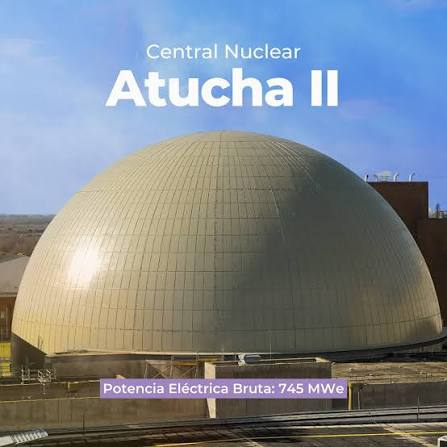
\includegraphics[width=\textwidth]{../Figures/cna2.jpg}
            % 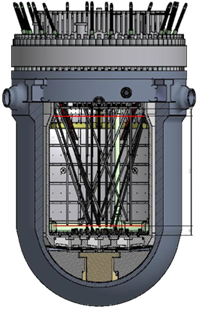
\includegraphics[width=\textwidth]{../Figures/cna2_rpv.png}
        \end{column}
    \end{columns}
\end{frame}

\begin{frame}
    \frametitle{Primero un poco de Ingeniería Nuclear...}
    Criterios de limitación de la potencia térmica.
    \begin{itemize}
        \item Fracción de vapor o vacío ($\alpha$) a la salida de los canales refrigerantes.
        \item Distancia al Apartamiento de la Ebullición Nucleada (DNBR, del inglés \textit{Departure from Nucleate Boiling Ratio}).
    \end{itemize}
    \begin{center}
        \resizebox{!}{0.6\textheight}{
            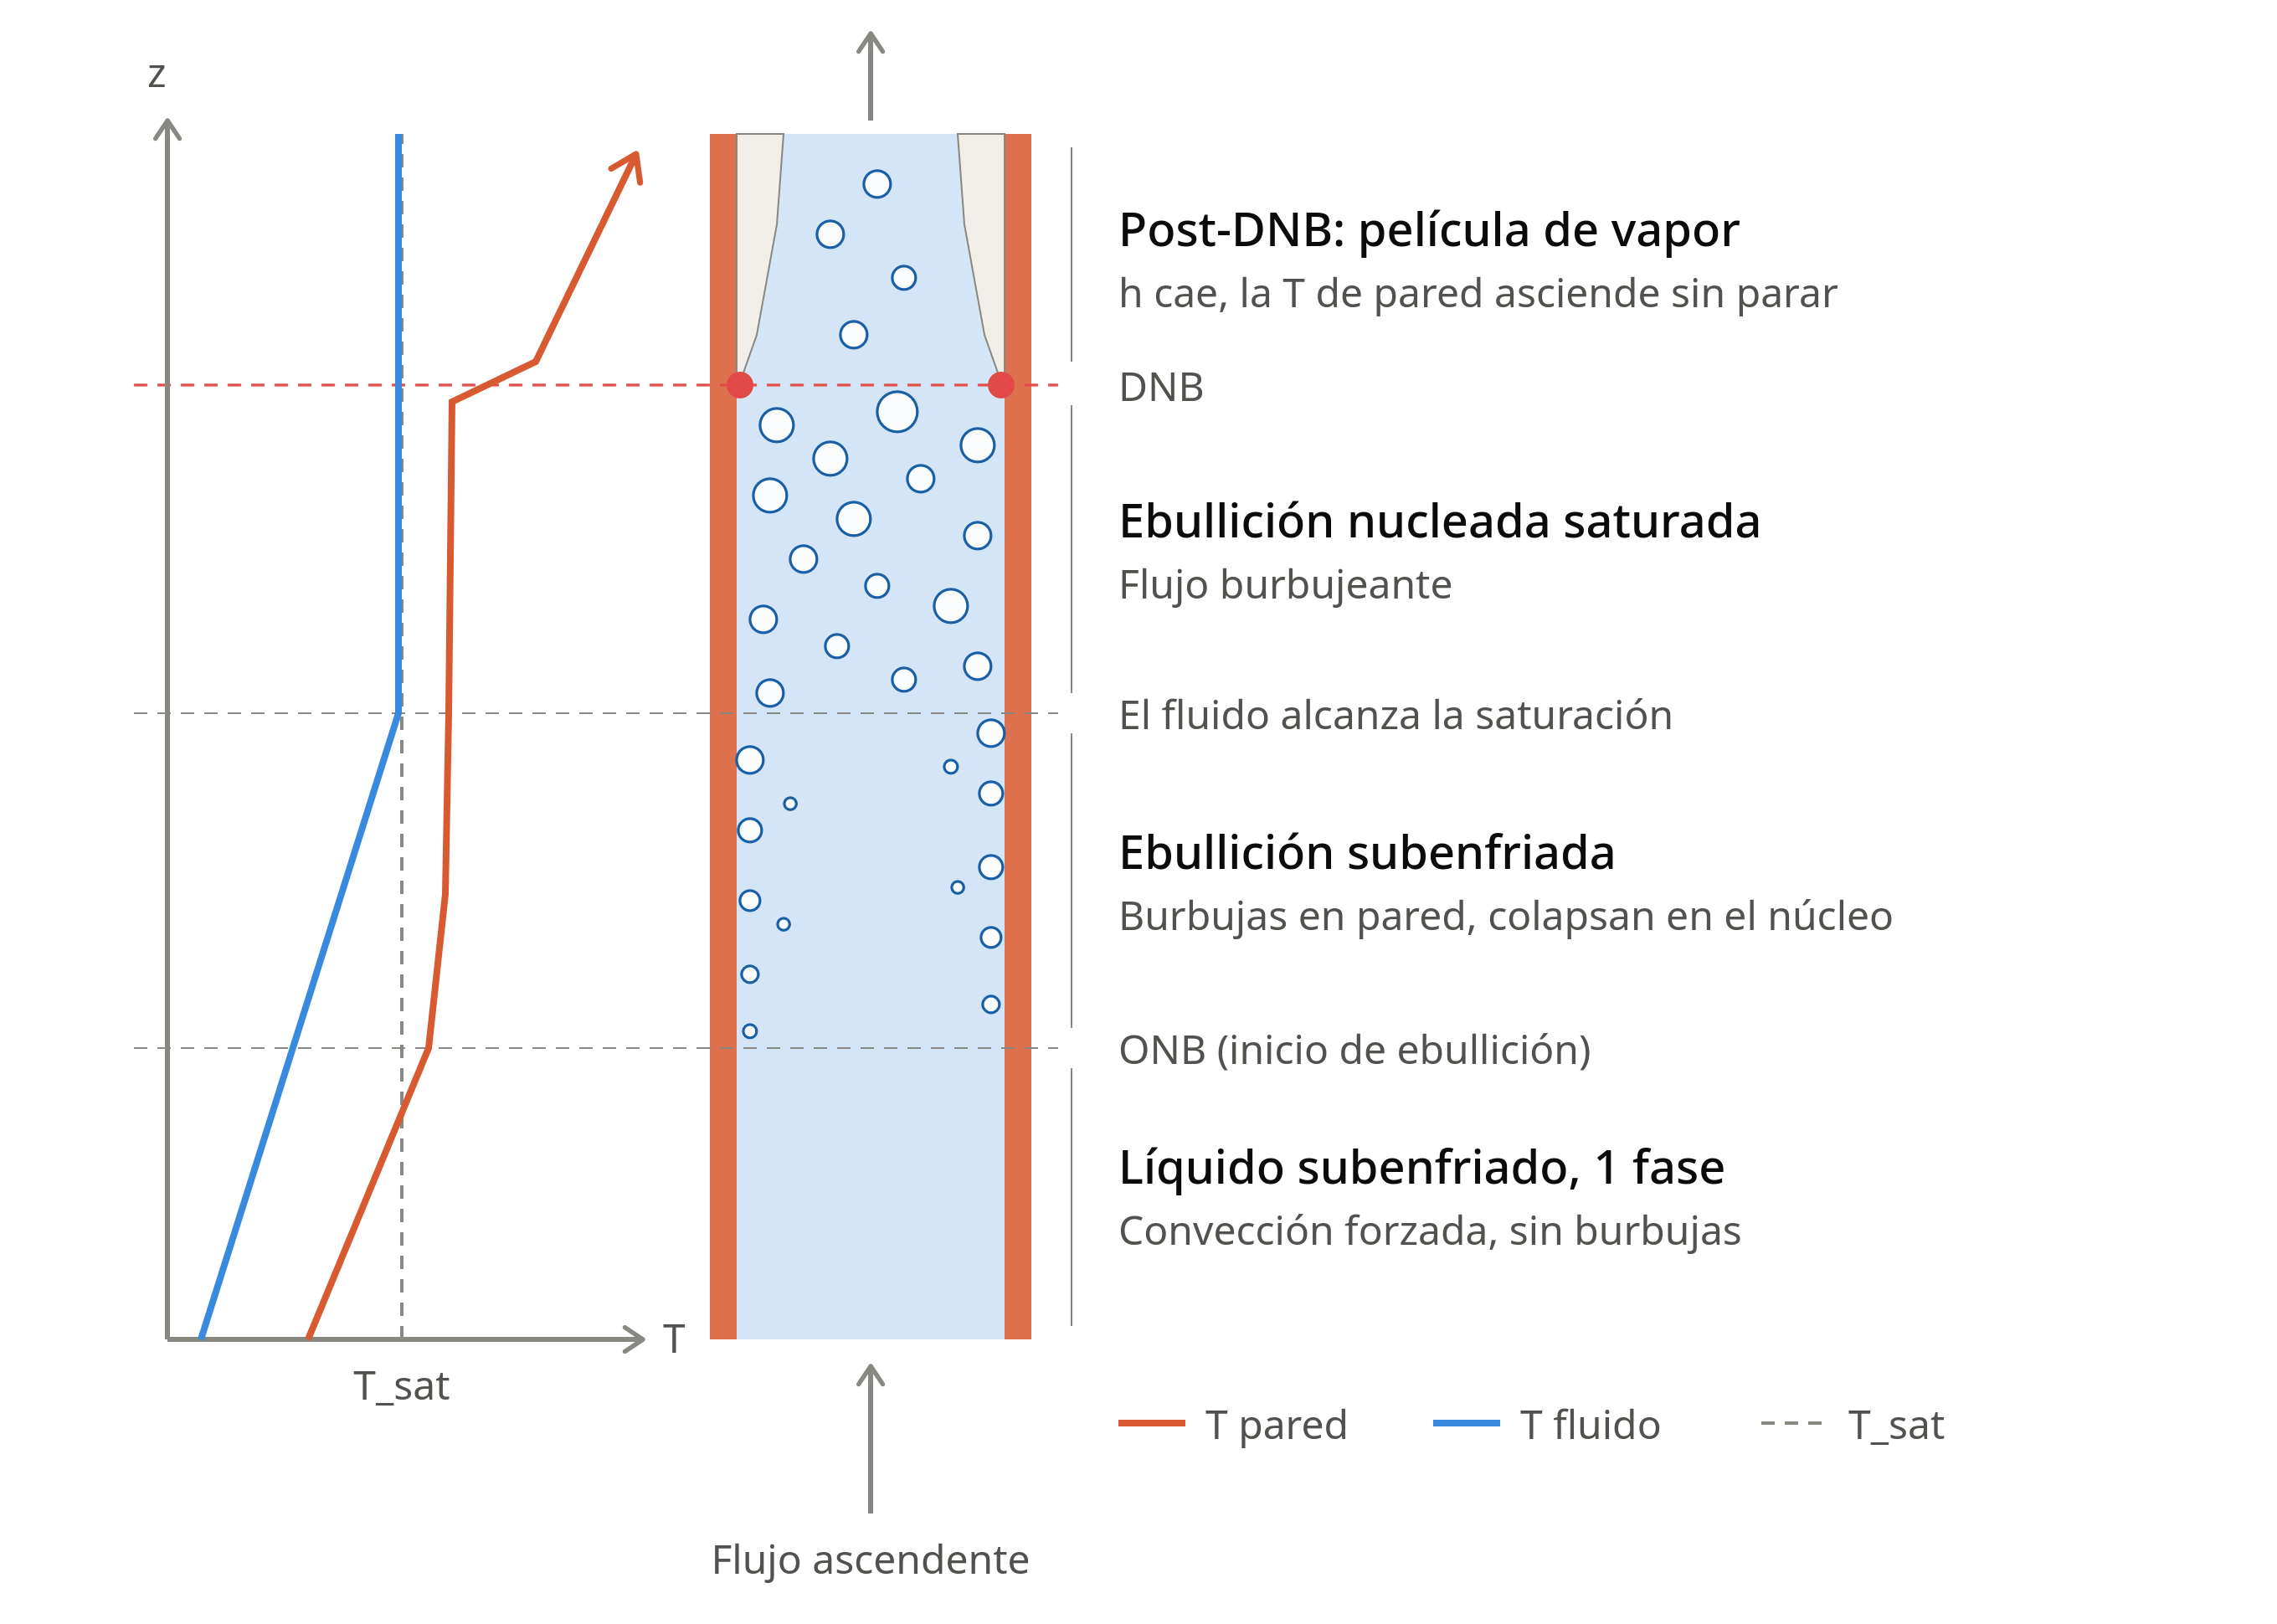
\includegraphics[width=\textwidth]{dnb_tubo_flujo_ascendente.png}
        }
    \end{center}
\end{frame}

\begin{frame}
    \frametitle{Primero un poco de Ingeniería Nuclear...}
    ¿Cuándo es necesario recalcular las potencias límite de canal (PLC)?
    \begin{itemize}
        \item Cambios de estrategia de recambio de combustible, cambios de condiciones de operación, operación con canales refrigerantes vacíos previo a parada programada, etc.
        \item Algunos casos pueden implicar más de 1 millón de cálculos individuales.
    \end{itemize}

    ¿Cómo se calculan las PLC?
    \begin{itemize}
        \item Código de subcanales COBRA-3CP, especialmente calibrado para la predicción de las condiciones termohidráulicas de los canales refrigerantes de la CNA-UII.
    \end{itemize}

    ¿Cómo se calcula la distancia al DNB o DNBR?
    \begin{itemize}
        \item Correlaciones de CHF en un tubo.
        \item Correcciones para la geometría de la CNA-UII a partir de ensayos experimentales.
    \end{itemize}
\end{frame}

% \begin{frame}
%     \frametitle{Apartamiento de la Ebullición Nucleada - DNB}
%     \begin{figure}
%         \centering
%         \resizebox{!}{0.85\textheight}{
%             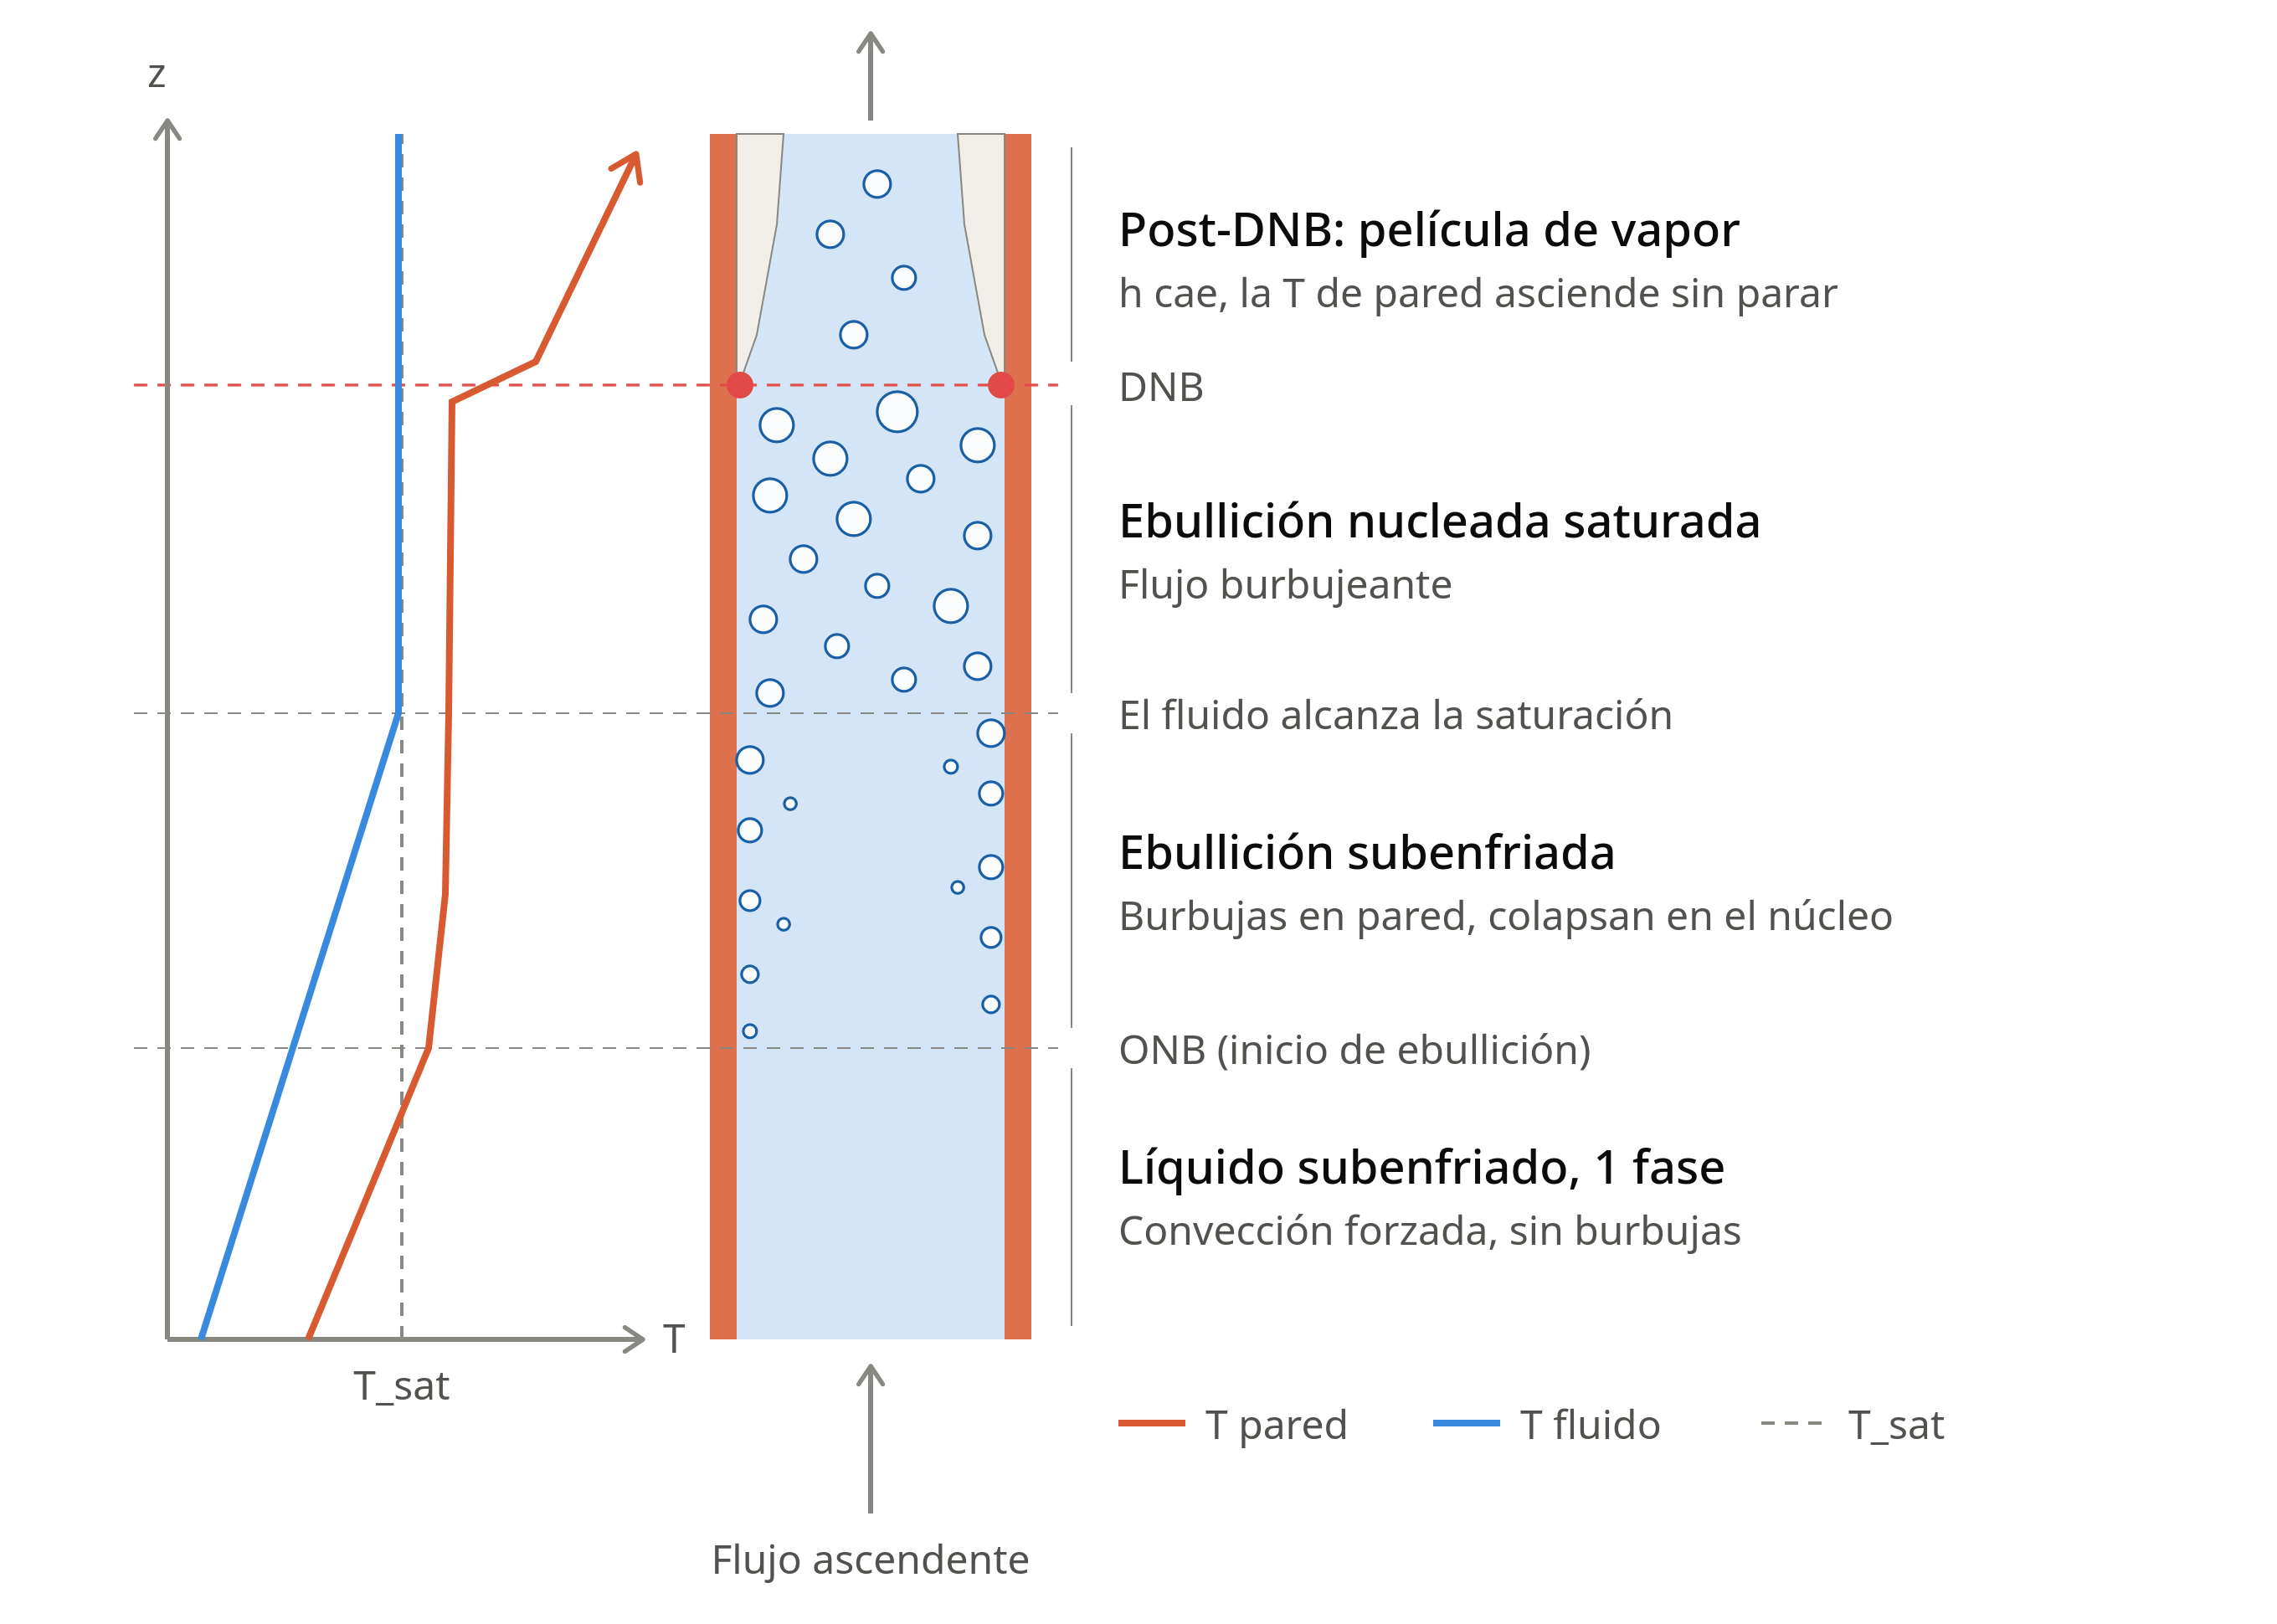
\includegraphics[width=\textwidth]{dnb_tubo_flujo_ascendente.png}
%         }
%     \end{figure}
% \end{frame}

\section{Contexto y motivación}

\begin{frame}
    \frametitle{IA + TH}
    \vspace{2cm}
    \begin{columns}
        \begin{column}{0.4\textwidth}
            \raggedleft
            {\Huge IA}
            \vspace{0.5cm}

            Inteligencia Artificial
        \end{column}
        \begin{column}{0.1\textwidth}
            \centering
            {\Huge +}
            \vspace{0.5cm}

            +
        \end{column}
        \begin{column}{0.4\textwidth}
            \raggedright
            {\Huge TH}
            \vspace{0.5cm}

           Termohidráulica 
        \end{column}

    \end{columns}
    \vspace{1cm}
    ¿Cómo puede la Inteligencia Artificial ayudar a la Termohidráulica Nuclear?
    \begin{itemize}
        \item Velocidad de predicción.
        \item Nuevas metodologías y mejores predicciones en campos de aplicación complejos. 
    \end{itemize}
\end{frame}

\begin{frame}
    \frametitle{Objetivos}
    Objetivos estratégicos:
    \begin{itemize}
        \item Disminuir el tiempo y costo computacional del cálculo de PLC, mantiendo precisión.
        \item Mejorar la precisión de la predicción de CHF para el bundle de la CNA-UII.
    \end{itemize}
    \vfill
    Objetivos específicos:
    \begin{enumerate}
        \item Desarrollar una herramienta predictiva de PLC por fracción de vapor y DNBR, entrenada con simulaciones de código de subcanales.
        \item Implementar reducción de dimensionalidad por medio de autoencoders para comprender las características relevantes de los perfiles de potencia de los elementos combustibles.
        \item Desarrollar una metodología basada en Inteligencia Artificial para mejorar la precisión de la predicción de CHF para el bundle de la CNA-UII.
    \end{enumerate}
\end{frame}

% \section{Introducción específica}
% \begin{frame}
%     \frametitle{Introducción específica}
    
% \end{frame}

\section{Predictor de PLC}
\begin{frame}
    \frametitle{Predictor de PLC}
    \textbf{¿Cómo se pueden aprovechar la IA para obtener mayor velocidad en el cálculo de PLC?}

    Cálculo de la fracción de vapor y el DNBR, a partir de condiciones termohidráulicas de entrada y perfiles de potencia de los elementos combustibles.
    \begin{itemize}
        \item Pocas variables de entrada.
        \item Muchos datos disponibles para entrenamiento.
        % \item Sencillo implementar un lazo de cálculo para obtener los límites de operación.
    \end{itemize}

    Una red neuronal profunda (DNN) puede aprender la relación entre las condiciones de entrada y los resultados de salida.

    Un lazo de cálculo iterativo permite utilizar la DNN para obtener las PLC según las condiciones. 
\end{frame}

\begin{frame}
    \frametitle{Predictor de PLC - Entrenamiento de la DNN}
    Conjunto de entrenamiento:
    \begin{itemize}
        \item Potencia entre $5\%$ y $30\%$ sobre nominal.
        \item Temperatura entre $268$ y $288$ °C ($\pm 10$ °C nominal).
        \item Presión entre $105$ y $125\,\mathrm{bar}$ ($\pm 10\,\mathrm{bar}$ nominal).
    \end{itemize}
    \begin{figure}[t]
        \centering 
        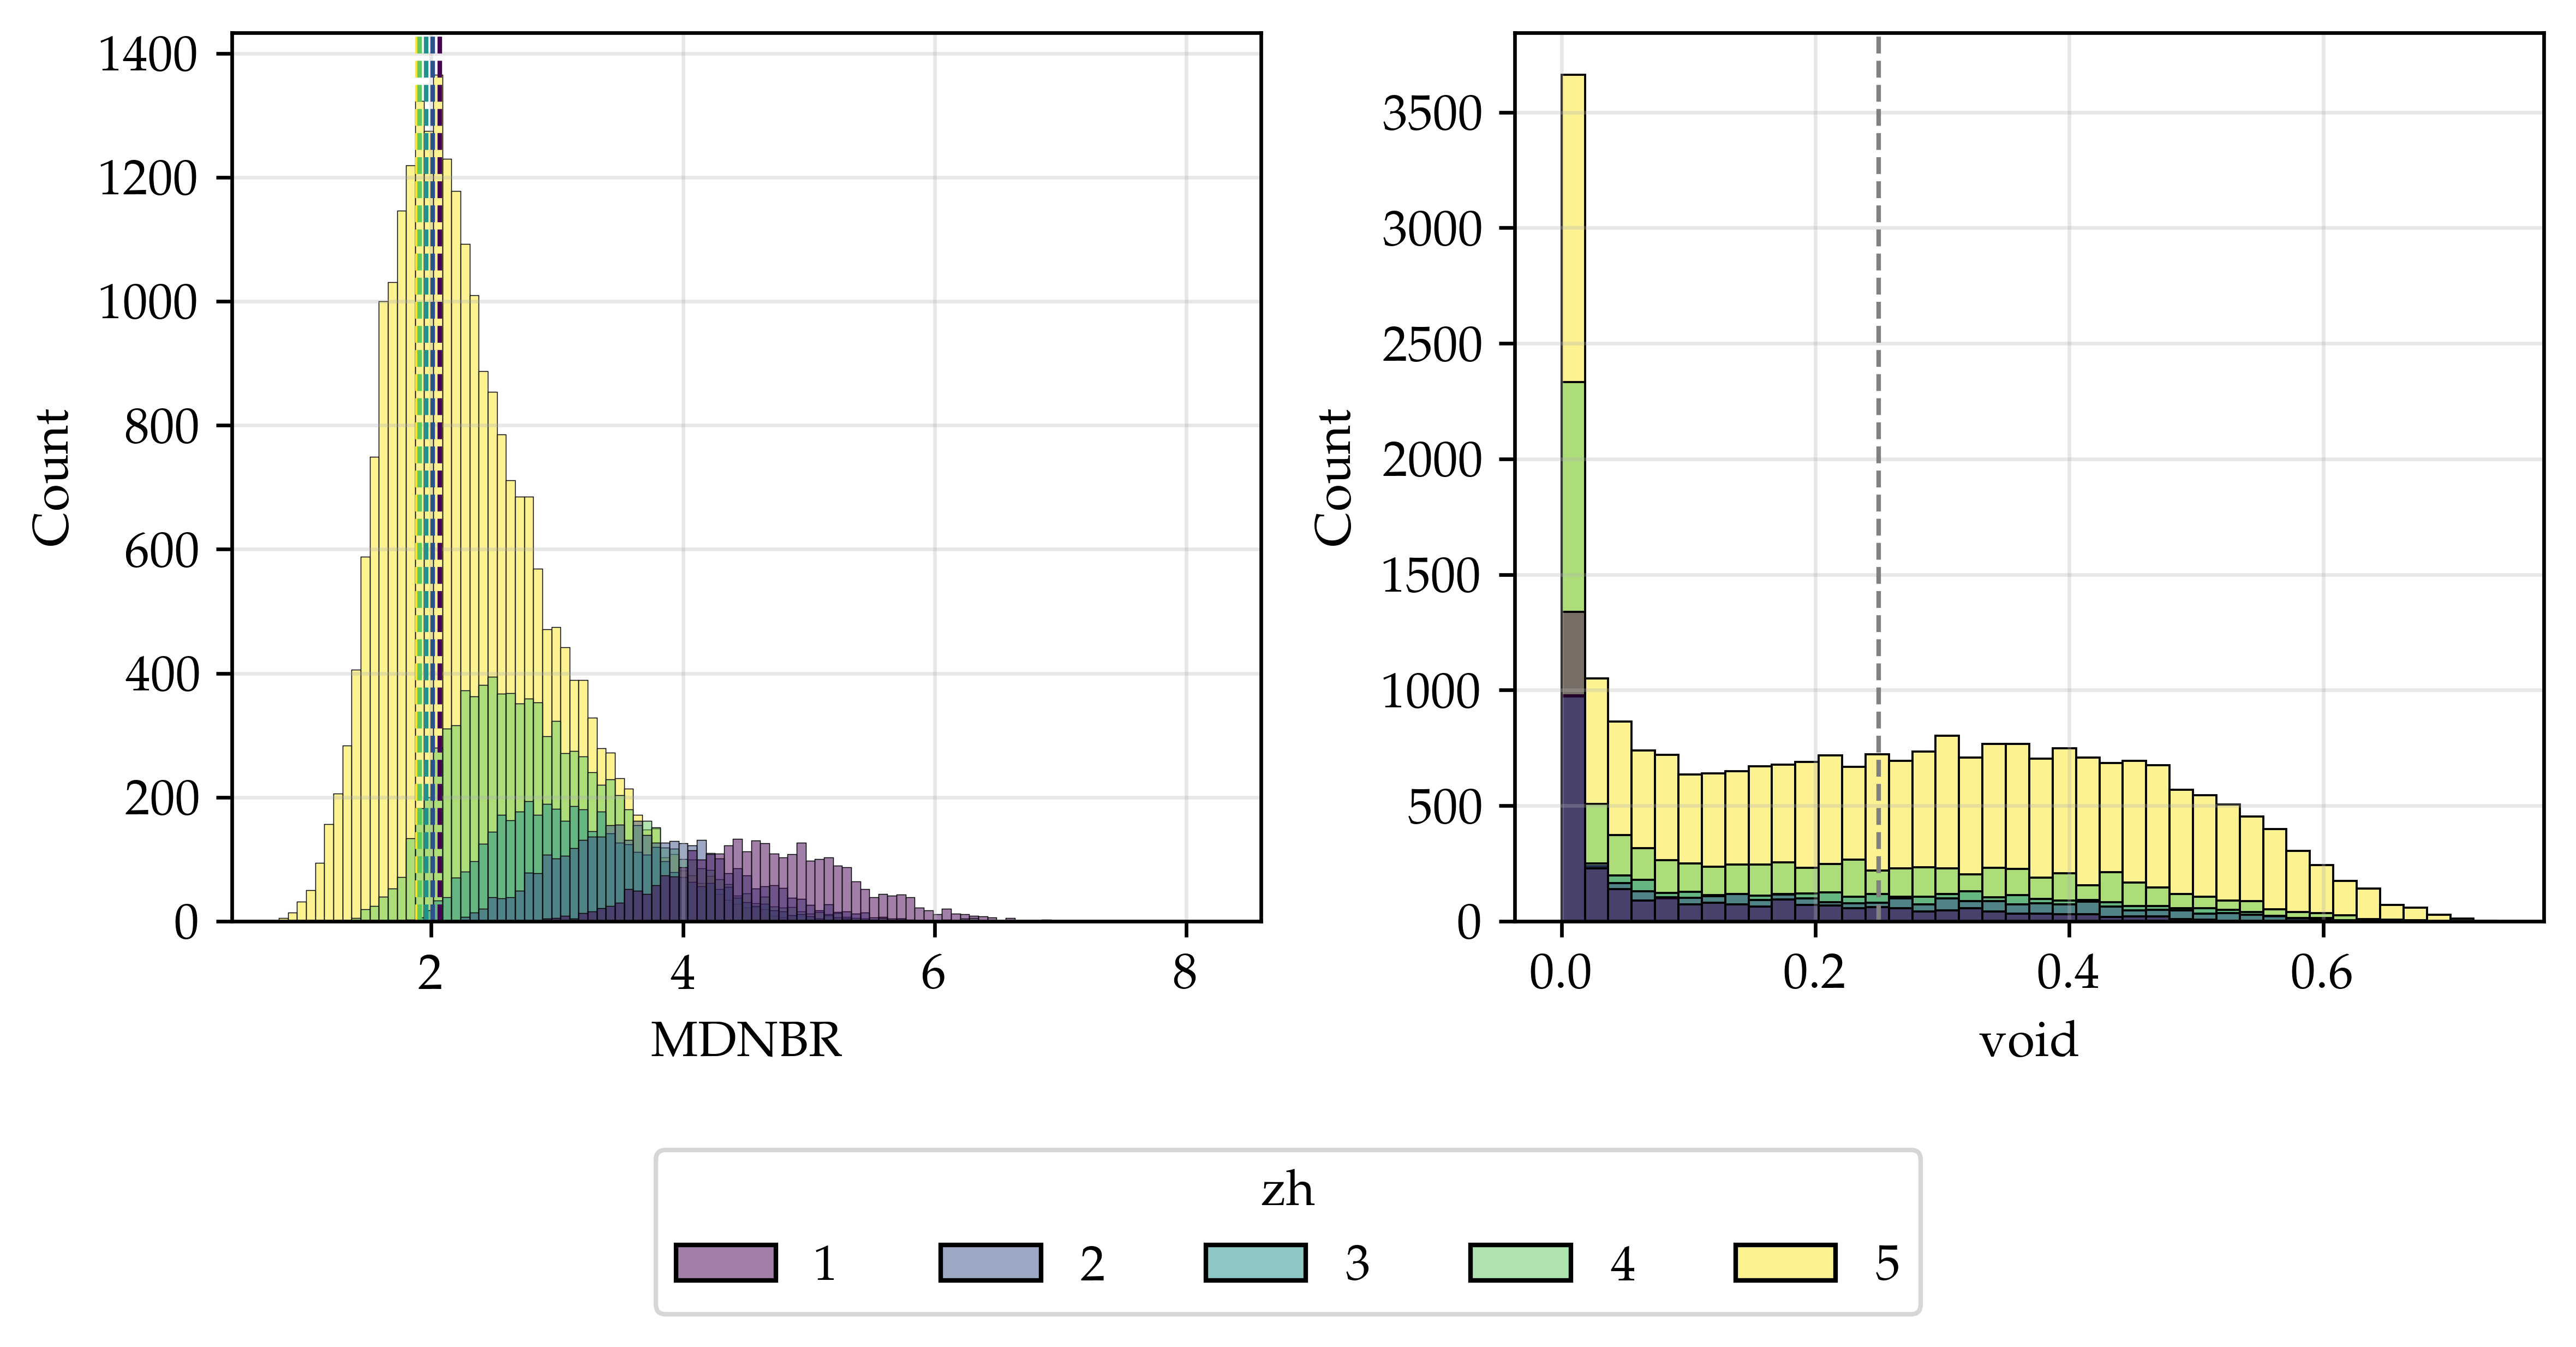
\includegraphics[width=0.85\textwidth]{plc_eda.png}
    \end{figure}
\end{frame}

% \begin{frame}
%     \frametitle{Predictor de PLC - Entrenamiento de la DNN}
%     \begin{itemize}
%         \item Optimizador: Adam.
%         \item Optimización de hiperparámetros con Optuna.
%         \item Función de pérdida: MRE para DNBR y $100\cdot$MAE para $\alpha$.
%     \end{itemize}
%     \vspace{0.5cm}
%     Hiperparámetros optimizados:
%     \begin{table}[H]
%         \small
%         \centering
%         % \caption{Hiperparámetros de la arquitectura final.}
%         \begin{tabular}{l c}    
%             \toprule
%             \textbf{Hiperparámetro} & \textbf{Valor} \\
%             \hline
%             Cantidad de capas ocultas & $3$ \\
%             Cantidad de neuronas por capa & $478$ \\
%             Learning rate & $1.38 \cdot 10^{-4}$ \\
%             Batch & 64 \\
%             Función de activación & ReLU \\
%             \bottomrule
%         \end{tabular}
%         % \label{tab:plc_arq_hp}
%     \end{table}

% \end{frame}

\begin{frame}
    \frametitle{Predictor de PLC - Resultados de predicción}

    \textbf{Predicción de DNBR:} subpredicción con media de $0.006$. Conservativo.

    \textbf{Predicción de la fracción de vacío:} sobrepredicción con media de $0.018$. Conservativo.

    \begin{figure}[t]
        \centering 
        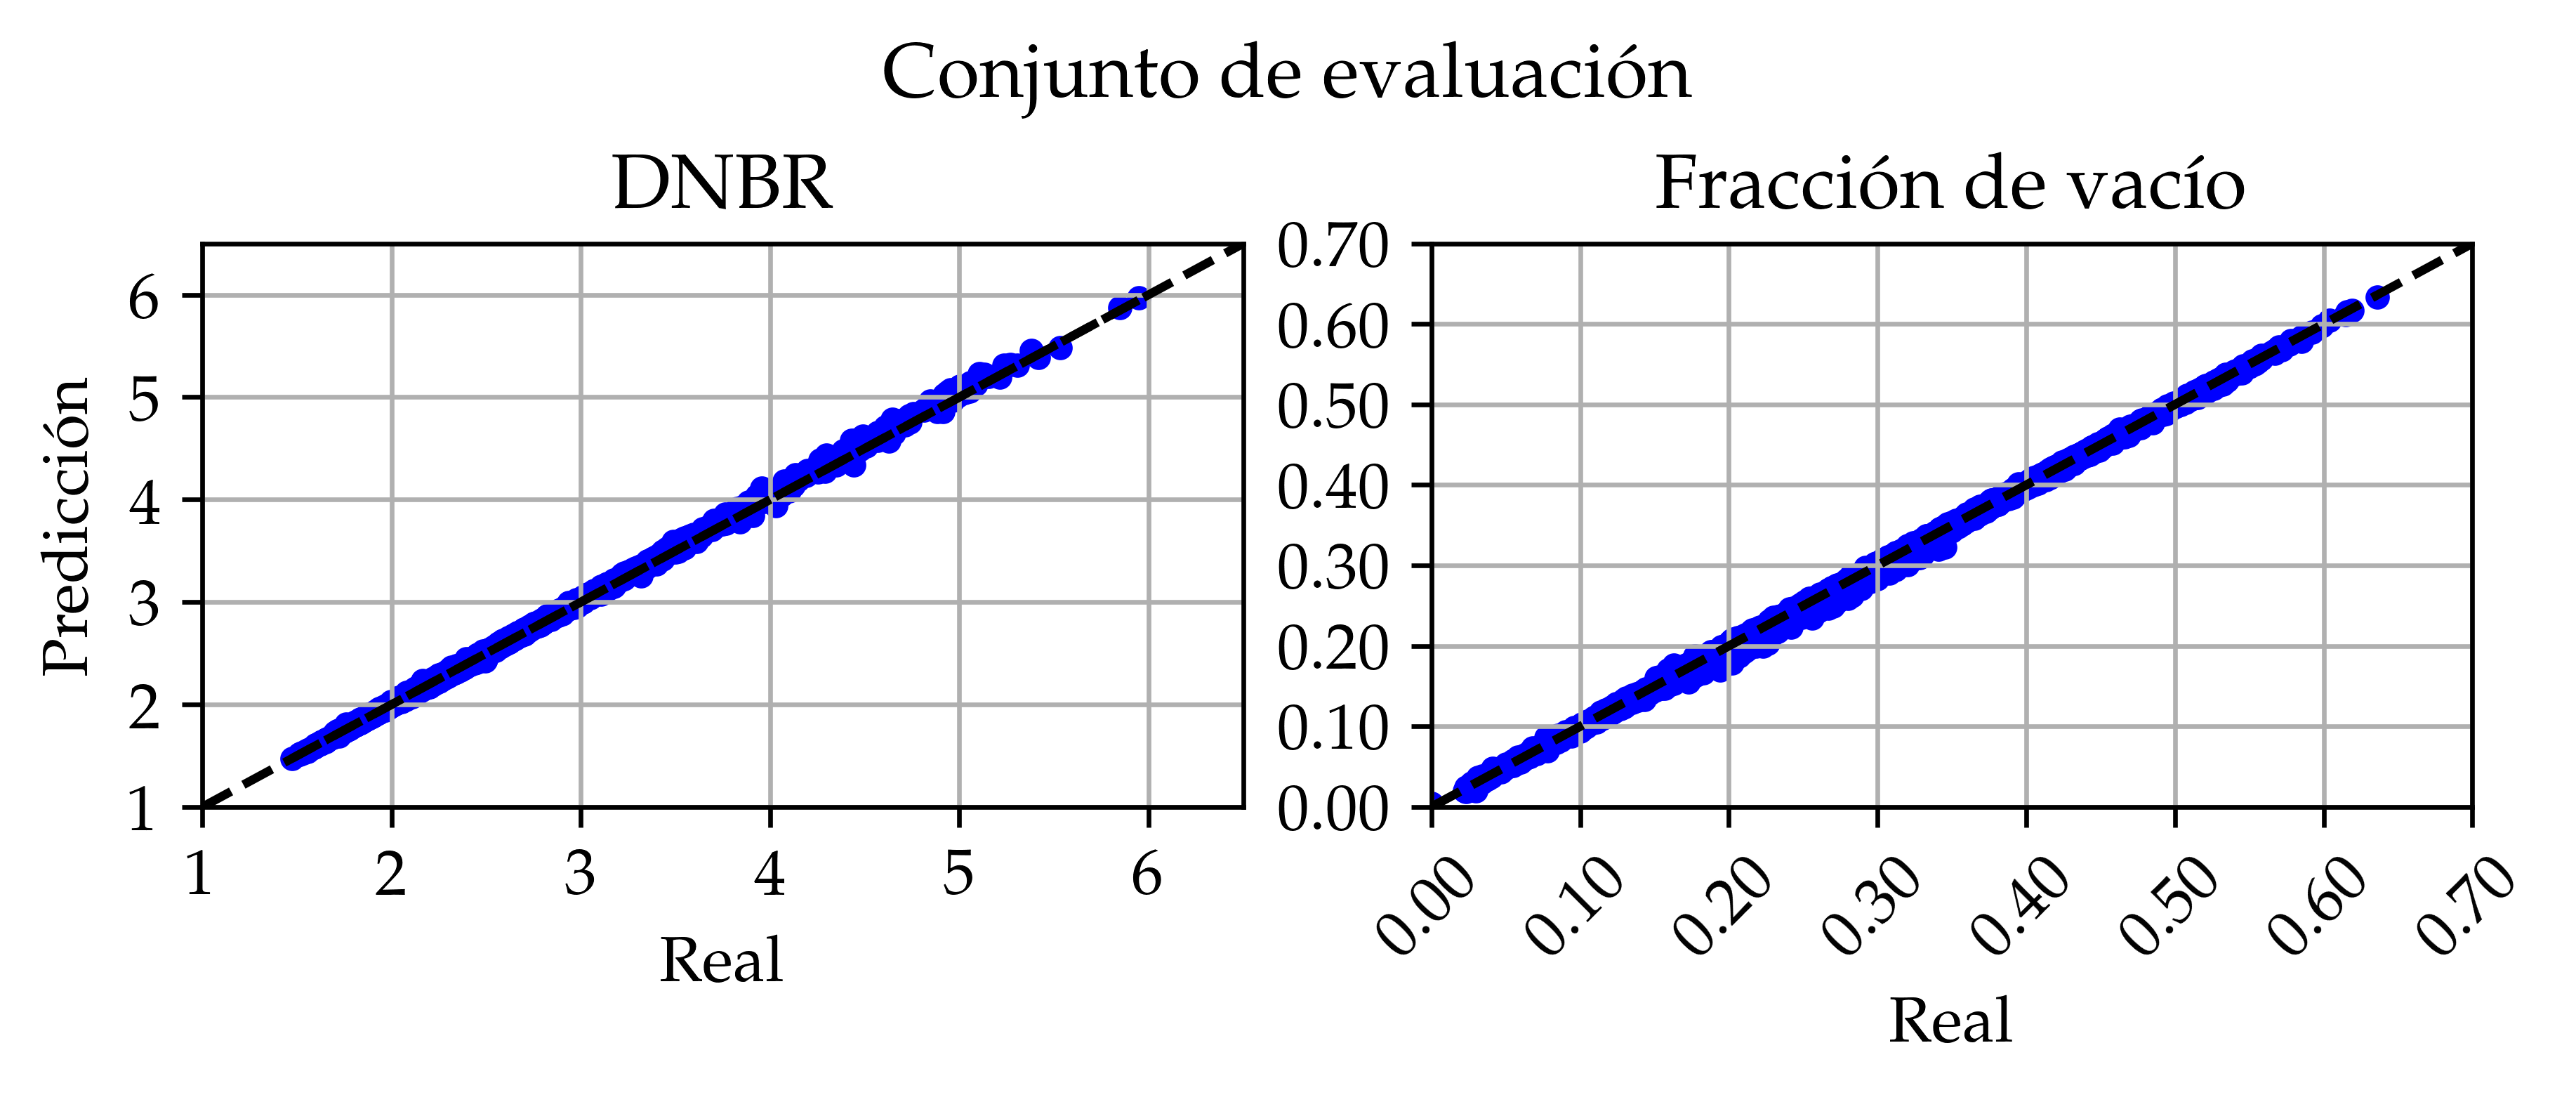
\includegraphics[width=0.9\textwidth]{plc_pred_test.png}
        % \caption{Resultados de predicción de la fracción de vapor y el DNBR para el conjunto de evaluación.}
    \end{figure}
\end{frame}

\begin{frame}
    \frametitle{Predictor de PLC - Lazo de cálculo}
    ¿Cómo estimar PLC a partir de la predicción de DNBR y fracción de vacío de la DNN?
    % % Versión simplificada del esquema del lazo de cálculo de la potencia límite por DNBR,
% pensada para una diapositiva de beamer.
% Requiere en el preámbulo:
%   \usepackage{tikz}
%   \usetikzlibrary{arrows.meta, positioning, shapes.geometric}
% Incluir en el frame con, por ejemplo:
%   \begin{frame}{Lazo de cálculo de la potencia límite por DNBR}
%       \centering
%       \input{Figures/loop_potencia_dnbr_beamer.tex}
%   \end{frame}
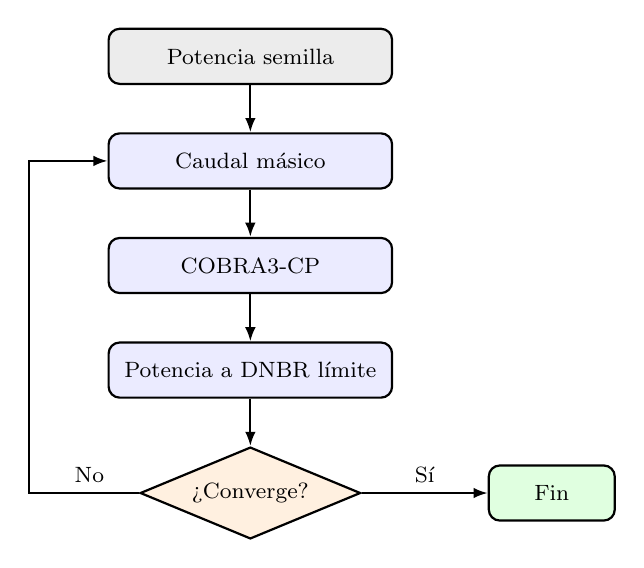
\begin{tikzpicture}[
    font=\footnotesize,
    arr/.style={-{Latex[length=1.8mm]}, thick},
    node distance=6mm and 12mm,
    box/.style={
        rectangle, rounded corners, draw, thick,
        fill=blue!8, align=center,
        text width=34mm, minimum height=7mm, inner sep=1mm
    },
    startbox/.style={box, fill=gray!15},
    decision/.style={
        diamond, draw, thick, fill=orange!12, aspect=2.4,
        align=center, text width=22mm, inner sep=0mm
    },
    endbox/.style={
        rectangle, rounded corners, draw, thick,
        fill=green!12, align=center,
        text width=14mm, minimum height=7mm, inner sep=1mm
    },
]

    % Flujo principal
    \node[startbox]                  (init)   {Potencia semilla};
    \node[box, below=of init]        (caudal) {Caudal másico};
    \node[box, below=of caudal]      (cobra)  {COBRA3-CP};
    \node[box, below=of cobra]       (extrae) {Potencia a DNBR límite};
    \node[decision, below=of extrae] (conv)   {¿Converge?};
    \node[endbox, right=16mm of conv] (fin)   {Fin};

    \draw[arr] (init)   -- (caudal);
    \draw[arr] (caudal) -- (cobra);
    \draw[arr] (cobra)  -- (extrae);
    \draw[arr] (extrae) -- (conv);
    \draw[arr] (conv)   -- node[above] {Sí} (fin);

    % Realimentación: si no converge, se repite el cálculo de caudal
    \coordinate (loop) at ([xshift=-10mm] caudal.west);
    \draw[arr] (conv.west) -- node[above, pos=0.45] {No} (loop |- conv.west)
        -- (loop) -- (caudal.west);

\end{tikzpicture}

    \vspace{0.5cm}

    \begin{columns}
        \begin{column}{0.6\textwidth}
            \centering
            \resizebox{!}{0.8\textwidth}{
                % Version simplificada del lazo de calculo del flujo de calor que alcanza el
% MDNBR objetivo, pensada para una diapositiva de beamer.
%
% Requiere en el preambulo:
%   \usepackage{tikz}
%   \usetikzlibrary{arrows.meta}
%   \usepackage{amsmath,amssymb}
%
% Incluir en el frame con, por ejemplo:
%   \begin{frame}{Lazo de calculo del flujo de calor}
%       \centering
%       \input{Figures/dnb_dnn_loop_beamer.tex}
%   \end{frame}
%
% Simplificaciones respecto de fig:dnb-dnn-loop: cada rama (piso y techo) se
% resume en una unica caja, los pasos 3.a y 3.b se agrupan en una sola caja, el
% criterio de convergencia se enuncia en palabras y el esquema en miniatura de
% la DNN aparece una sola vez.

\resizebox{!}{0.78\textheight}{%
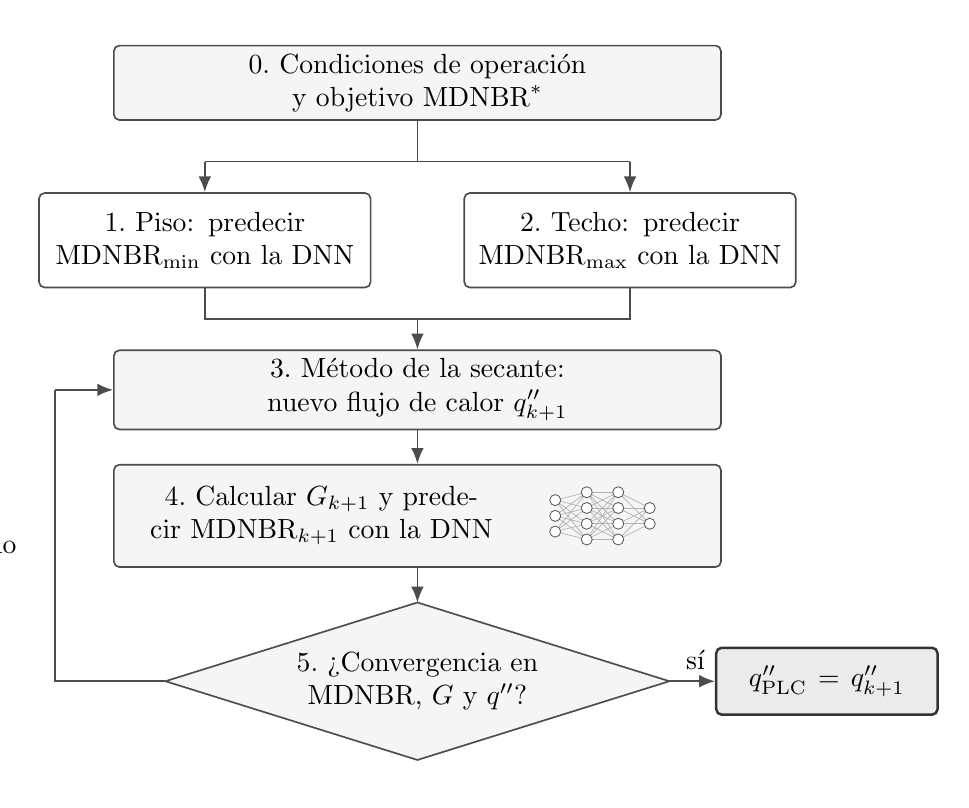
\begin{tikzpicture}[
    caja/.style   = {rectangle, rounded corners=2pt, draw=black!70,
                     fill=black!4, line width=0.6pt, text width=7.5cm,
                    %  align=center, font=\footnotesize, minimum height=0.9cm,
                     align=center, font=\normalsize, minimum height=0.9cm,
                     inner sep=3pt},
    subcaja/.style= {rectangle, rounded corners=2pt, draw=black!70,
                     fill=white, line width=0.6pt, text width=4cm,
                    %  align=center, font=\footnotesize, minimum height=1.2cm,
                     align=center, font=\normalsize, minimum height=1.2cm,
                     inner sep=3pt},
    final/.style  = {rectangle, rounded corners=2pt, draw=black!80,
                     fill=black!8, line width=0.9pt, text width=2.6cm,
                    %  align=center, font=\footnotesize, minimum height=0.85cm,
                     align=center, font=\normalsize, minimum height=0.85cm,
                     inner sep=3pt},
    rombo/.style  = {draw=black!70, fill=black!4, line width=0.6pt},
    % texto/.style  = {font=\footnotesize, align=center, inner sep=1pt},
    % nombre/.style = {font=\footnotesize, inner sep=1pt},
    texto/.style  = {font=\normalsize, align=center, inner sep=1pt},
    nombre/.style = {font=\normalsize, inner sep=1pt},
    flecha/.style = {-{Latex[length=2mm,width=1.6mm]}, draw=black!70,
                     line width=0.6pt},
    linea/.style  = {draw=black!70, line width=0.6pt},
    %--- estilos del esquema en miniatura de la red
    nnnodo/.style = {circle, draw=black!65, fill=white, line width=0.3pt,
                     minimum size=1.4mm, inner sep=0pt},
    nnarco/.style = {draw=black!30, line width=0.25pt},
    %--- esquema en miniatura de la DNN (3 entradas, 4+4 ocultas, 2 salidas)
    dnnmini/.pic  = {
      \foreach \ya in {0.20,0,-0.20}
        \foreach \yb in {0.30,0.10,-0.10,-0.30}
          \draw[nnarco] (0,\ya) -- (0.4,\yb);
      \foreach \ya in {0.30,0.10,-0.10,-0.30}
        \foreach \yb in {0.30,0.10,-0.10,-0.30}
          \draw[nnarco] (0.4,\ya) -- (0.8,\yb);
      \foreach \ya in {0.30,0.10,-0.10,-0.30}
        \foreach \yb in {0.10,-0.10}
          \draw[nnarco] (0.8,\ya) -- (1.2,\yb);
      \foreach \y in {0.20,0,-0.20}
        \node[nnnodo] at (0,\y) {};
      \foreach \y in {0.30,0.10,-0.10,-0.30} {
        \node[nnnodo] at (0.4,\y) {};
        \node[nnnodo] at (0.8,\y) {};
      }
      \foreach \y in {0.10,-0.10}
        \node[nnnodo] at (1.2,\y) {};
    },
  ]
  \useasboundingbox (-4.95,-8.85) rectangle (6.65,0.70);

  %-------------------------------------------------- 0. condiciones
  \node[caja] (A) at (0,0)
    {0.~Condiciones de operaci\'on\\y objetivo $\mathrm{MDNBR}^{*}$};

  %-------------------------------------------------- 1 y 2. piso y techo
  \node[subcaja] (P) at (-2.7,-2.0)
    {1.~Piso: predecir $\mathrm{MDNBR}_{\min}$ con la DNN};
  \node[subcaja] (T) at ( 2.7,-2.0)
    {2.~Techo: predecir $\mathrm{MDNBR}_{\max}$ con la DNN};

  %-------------------------------------------------- 3. lazo de la secante
  \node[caja] (C) at (0,-3.90)
    {3.~M\'etodo de la secante:\\nuevo flujo de calor $q''_{k+1}$};

  \node[caja, minimum height=1.3cm] (D) at (0,-5.50) {};
  \node[texto, text width=6cm] at (-1.22,-5.50)
    {4.~Calcular $G_{k+1}$ y predecir $\mathrm{MDNBR}_{k+1}$ con la DNN};
  \pic at (1.75,-5.50) {dnnmini};

  %-------------------------------------------------- convergencia
  \draw[rombo] (0,-6.60) -- (3.2,-7.60) -- (0,-8.60) -- (-3.2,-7.60) -- cycle;
  \node[texto, text width=4.0cm] at (0,-7.60)
    {5.~\textrm{\textquestiondown}Convergencia en\\
     $\mathrm{MDNBR}$, $G$ y $q''$?};

  \node[final] (F) at (5.20,-7.60) {$q''_{\mathrm{PLC}}=q''_{k+1}$};

  %-------------------------------------------------- flujo: 0 -> ramas
  \draw[linea]  (A.south) -- (0,-1.00);
  \draw[linea]  (-2.7,-1.00) -- (2.7,-1.00);
  \draw[flecha] (-2.7,-1.00) -- (P.north);
  \draw[flecha] ( 2.7,-1.00) -- (T.north);

  %-------------------------------------------------- ramas -> secante
  \draw[linea]  (P.south) -- (-2.7,-3.0) -- (0,-3.00);
  \draw[linea]  (T.south) -- ( 2.7,-3.0) -- (0,-3.00);
  \draw[flecha] (0,-3.00) -- (C.north);

  %-------------------------------------------------- lazo
  \draw[flecha] (C.south) -- (D.north);
  \draw[flecha] (D.south) -- (0,-6.60);

  \draw[flecha] (3.2,-7.60) -- (F.west);
  \node[nombre] at (3.53,-7.33) {s\'i};

  \draw[linea]  (-3.2,-7.60) -- (-4.6,-7.60) -- (-4.6,-3.90);
  \draw[flecha] (-4.6,-3.90) -- (C.west);
  \node[nombre, anchor=east] at (-5.05,-5.90) {no};
\end{tikzpicture}}

            }
        \end{column}
        \begin{column}{0.4\textwidth}
            Factor de corrección para asegurar con 95\% de probabilidad y confianza subpredicción de PLC.
            \begin{equation*}
                \mathrm{PLC}^* = \mathrm{PLC} \cdot F_\mathrm{PLC}
            \end{equation*}
            \begin{table}
                \centering
                \small
                \begin{tabular}{l c c} 
                    \toprule 
                    \multirow{2}{*}{ZH} & \multicolumn{2}{c}{$F_\mathrm{PLC}$} \\
                    & DNBR & $\alpha$ \\ \hline
                    1 & $0.933$ & $0.985$ \\
                    5 & $0.995$ & $0.997$ \\
                    \bottomrule
                \end{tabular}
            \end{table}
        \end{column}
    \end{columns}
\end{frame}

% \begin{frame}
%     \frametitle{Predictor de PLC - Corrección conservadora}

%     Factor de corrección para asegurar con 95\% de probabilidad y confianza que la PLC estimada por la DNN es conservativa respecto de la PLC calculada por COBRA3-CP.
%     \begin{equation}
%         \mathrm{PLC}^* = \mathrm{PLC} \cdot F_\mathrm{PLC}
%     \end{equation}
% \end{frame}

\begin{frame}
    \frametitle{Predictor de PLC - Resultados de predicción de PLC}
    Errores medios de predicción de PLC por DNBR y por fracción de vacío.
    \begin{table}
        \centering
        \small
        \begin{tabular}{l c c} 
            \toprule 
            \multirow{2}{*}{ZH} & \multicolumn{2}{c}{Media del error} \\
            & DNBR & $\alpha$ \\ \hline
            1 & $1.047$ & $1.008$ \\
            3 & $1.018$ & $1.002$ \\
            5 & $1.001$ & $1.001$ \\
            \bottomrule
        \end{tabular}
    \end{table}
    
    Predicciones con y sin corrección para la ZH5.
    \begin{figure}[t]
        \centering 
        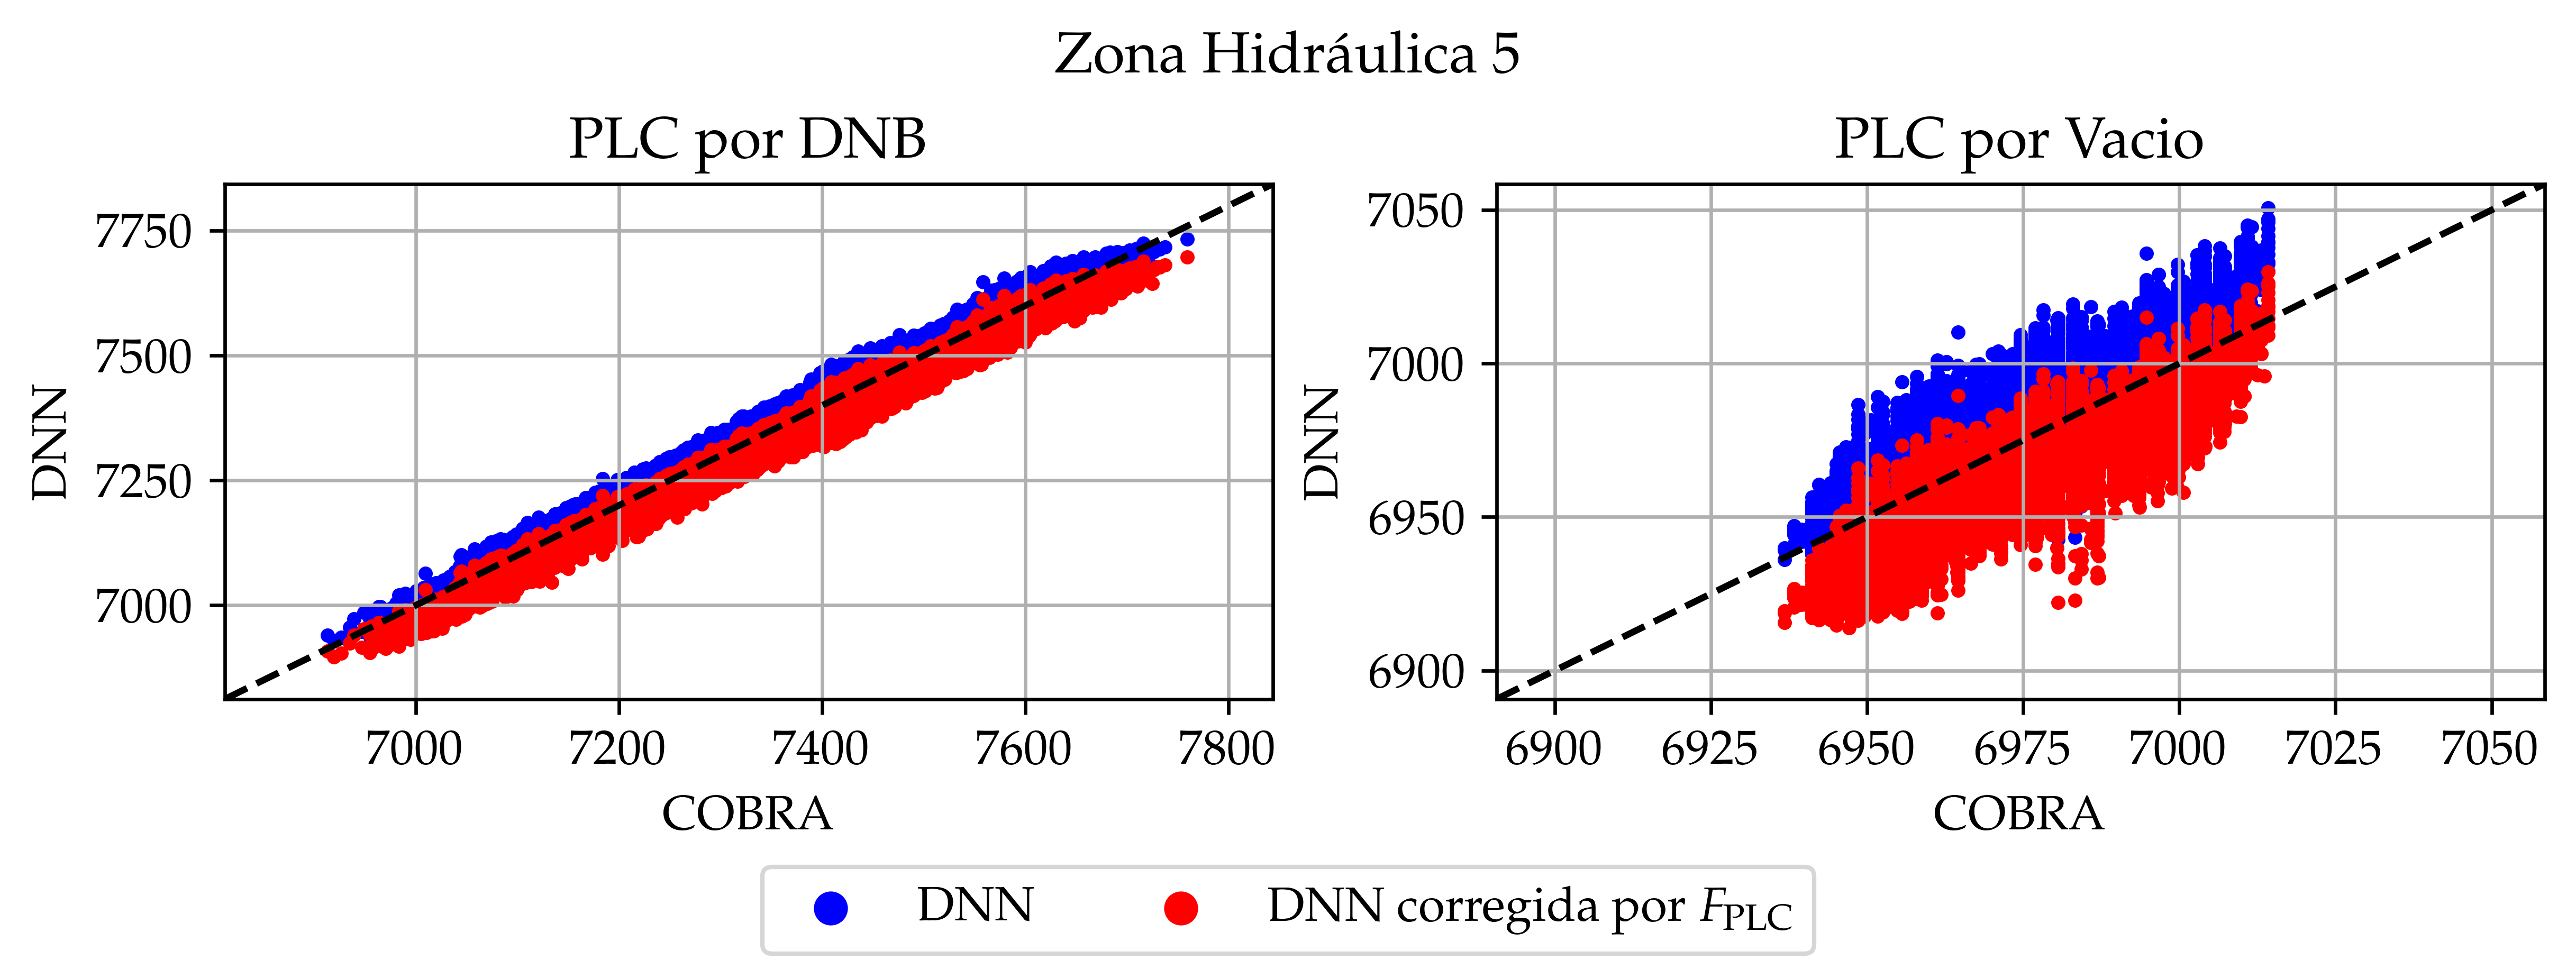
\includegraphics[width=0.85\textwidth]{plc_pred_loop_zh5.png}
        % \caption{Resultados de predicción de la fracción de vapor y el DNBR para el conjunto de evaluación.}
    \end{figure}
\end{frame}

\begin{frame}
    \frametitle{Predictor de PLC - Tiempos de cómputo}
    Se estimó la PLC por DNBR y fracción de vacío para 100 estados del reactor. 
    
    Aproximadamente un 4\% de una estrategia de recambio de combustible completa.

    \textbf{DNBR:} mejora de tiempo de cómputo entre $8\,500$ y $9\,500$ veces menor.

    \textbf{Fracción de vacío:} mejora de tiempo de cómputo entre $2\,000$ y $2\,500$ veces menor.

    \begin{table}[H]
        \centering
        \small
        % \caption{Tiempos de cómputo para cálculo de PLC.}
        \begin{tabular}{l c c c c c} 
            \toprule 
            % \multicolumn{6}{c}{Estimación de PLC para 100 estados del reactor.}
            % \\ \hline
            & \multicolumn{3}{c}{\textbf{Tiempo}} & \multicolumn{2}{c}{\multirow{2}{*}{\textbf{Mejora}}} \\
            & \multirow{2}{*}{\textbf{COBRA3-CP}} & \multicolumn{2}{c}{\textbf{DNN}} &  \\
            &                                     & CPU & GPU & CPU & GPU \\
            \hline
            DNBR   & 306 h     & 117 s & 130 s& x9 445  & x8 503\\
            \hline
            Fracción de vacío  & 74 h     & 108 s & 120 s & x2 479  & x2 224\\
            \bottomrule
        \end{tabular}
    \end{table}
\end{frame}

\section{Espacio latente de perfiles de potencia}
\begin{frame}
    \frametitle{Espacio latente de perfiles de potencia}
    \textbf{¿Cómo se pueden aprovechar la IA para comprender las características relevantes de los perfiles de potencia de los elementos combustibles?} 

    Autoencoder.

    \begin{figure}[H]
        \centering
        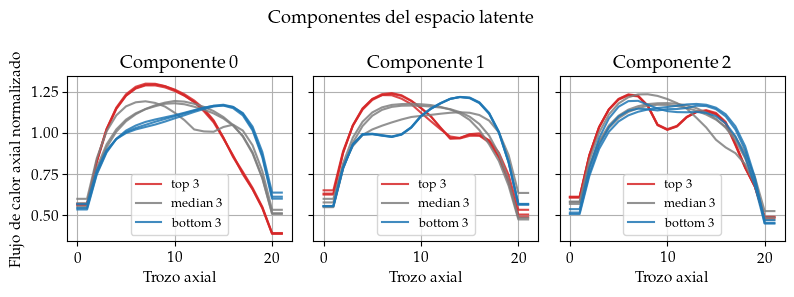
\includegraphics[trim=20 20 0 30,clip,width=0.8\textwidth]{../Figures/embeddings_axial_componentes_latente.png}
    % \end{figure}

    % \begin{figure}[hbtp]
    %     \centering
        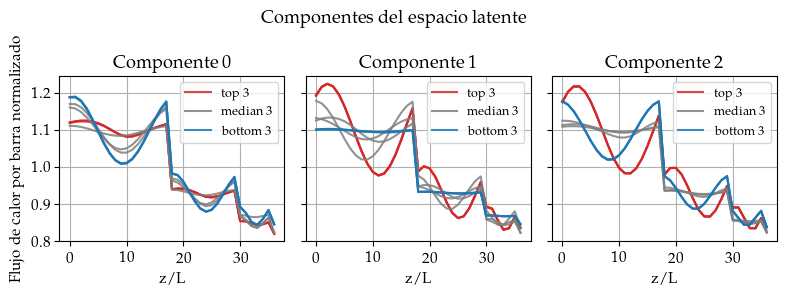
\includegraphics[trim=20 20 0 30,clip,width=0.8\textwidth]{../Figures/embeddings_radial_componentes_latente.png}
    \end{figure}


    
\end{frame}

\section{Predictor de CHF}

% \begin{frame}
%     \frametitle{Definición del enfoque}
%     Conjuntos de datos disponibles:
%     \begin{itemize}
%         \item Ensayos experimentales de CHF en tubos, recopilados por Groeneveld $\Longrightarrow$ alta disponibilidad, no representan la geometría de interés.
%         \item Ensayos experimentales de CHF en bundle de la CNA-UII, realizados por la UColumbia $\Longrightarrow$ baja disponibilidad de ensayos y de puntos medidos.
%         \item Replicación numérica con COBRA-3CP de los ensayos experimentales de CHF en bundle de la CNA-UII $\Longrightarrow$ pocos ensayos pero se tienen datos de todos los puntos, sujeto a error por los modelos implementados en COBRA-3CP.
%     \end{itemize}

%     Características adicionales del problema:
%     \begin{itemize}
%         \item No se tiene una ecuación de conservación a resolver.
%         \item Se tienen tendencias físicas conocidas y validadas con datos experimentales.
%         \item Los ensayos no reportan la ubicación de la ocurrencia de CHF.
%     \end{itemize}
% \end{frame}

\begin{frame}
    \frametitle{Definición del enfoque}
    Conjuntos de datos disponibles:
    \begin{table}[H]
        \centering
        \small
        % \caption{Tiempos de cómputo para cálculo de PLC.}
        \begin{tabular}{l l} 
            % \toprule 
            \multirow{2}{3.5cm}{Ensayos en tubo} & Alta disponibilidad \\
            & No representan la geometría de interés \\ \hline
            \multirow{3}{3.5cm}{Ensayos en bundle CNA-UII} & Baja disponibilidad \\
            & Representan la geometría de interés \\
            & No informan la ubicación de CHF \\ \hline
            \multirow{3}{3.5cm}{Replicación de ensayos con COBRA-3CP} & Baja disponibilidad de ensayos \\
            & Alta disponibilidad de puntos medidos \\
            & Representan la geometría de interés \\
            & No informan CHF
        \end{tabular}
    \end{table}

    Características adicionales del problema:
    \begin{itemize}
        \item No se tiene una ecuación de conservación a resolver.
        \item Se tienen tendencias físicas conocidas y validadas con datos experimentales.
        \item Los ensayos no reportan la ubicación de la ocurrencia de CHF.
    \end{itemize}
\end{frame}

\begin{frame}
    \frametitle{Definición del enfoque}
    \textbf{¿Cómo se puede aprovechar la IA considerando las limitaciones que impone el problema de predecir CHF para la CNA-UII?}

    \vfill

    Combinación de 2 conceptos:
    \begin{itemize}
        \item Redes Neuronales de \textbf{Multifidelidad} (MFNN). 
        \begin{itemize}
            \item Red de baja fidelidad (LFNN) predice CHF en tubos, a partir de condiciones locales.
            \item Red de alta fidelidad (HFNN) predice CHF en bundle de la CNA-UII, a partir de condiciones locales y la predicción de la LFNN.
        \end{itemize}
        \item Redes Neuronales \textbf{Informadas por Física} (PINN).
        \begin{itemize}
            \item Relaciones diferenciales del CHF con las condiciones locales.
            \item A partir de los ensayos en tubo.
        \end{itemize}
    \end{itemize}
    
\end{frame}

\begin{frame}
    \frametitle{Arquitectura MFPINN}
    \centering
    \resizebox{!}{0.82\textheight}{
        % Red neuronal multifidelidad:
%   - red de baja fidelidad (BF) pre-entrenada, con pesos fijos, que usa solo el
%     subconjunto de entradas x_1..x_n;
%   - red de alta fidelidad (AF) informada por la fisica (PINN), que usa todas las
%     entradas x_1..x_N mas la prediccion u_BF.
% La columna de entradas se dibuja UNA sola vez y es compartida: las entradas del
% subconjunto (recuadro sombreado) salen dos veces, hacia la red BF y hacia el bus
% de todas las entradas, mientras que las restantes salen solo hacia el bus.
%
% Fragmento para \input directo (sin el paquete standalone).
% NO necesita ninguna libreria de TikZ: solo \usepackage{tikz} y \usepackage{amsmath}.
% Uso tipico:
%   \begin{figure}[htbp]\centering
%     \resizebox{\textwidth}{!}{\input{Figures/mfnn_pinn.tex}}
%     \caption{...}\label{fig:mfnn_pinn}
%   \end{figure}
%
% Notas de implementacion (todas para que el fragmento no dependa del preambulo):
%  - Sin \usetikzlibrary aqui adentro: ejecutado en modo horizontal (dentro de un
%    \resizebox) deja ~55pt de espacios que ensanchan la caja del \input y hacen que
%    \resizebox empequenezca el dibujo; y no se puede encerrar en un grupo o \hbox
%    para absorberlos porque las definiciones de las librerias son locales.
%  - Sin la libreria backgrounds: los recuadros de las entradas y las conexiones van
%    en una capa `fondo` declarada con pgf basico (\pgfdeclarelayer), debajo de los
%    circulos rellenos de blanco.
%  - Sin la libreria fit: los recuadros de las redes se dan por coordenadas explicitas.
%  - Sin la libreria arrows.meta: las puntas son `stealth`, que ya trae pgf. Ademas se
%    escriben como -stealth y no con la clave >=, para no depender de que babel-spanish
%    tenga desactivado el shorthand `>`.
%  - Los tamanos de fuente son absolutos (\fontsize) para que la geometria no dependa
%    del tamano base del documento que hace el \input.
%  - Version compacta para beamer (~11.6 x 9.5 cm) con fuentes de 12pt, para que al
%    escalarla a la altura del frame las etiquetas sigan siendo legibles.
% \begin{figure}[hbtp!]
% \begin{figure}[H]
%   \centering
  % \resizebox{\textwidth}{!}{
\begin{tikzpicture}[
  chico/.style={font=\fontsize{12}{14}\selectfont},
  % un unico estilo de circulo: entradas, neuronas y salidas miden todas lo mismo
  entrada/.style={circle,draw=black!70,fill=white,minimum size=0.7cm,inner sep=0pt,
                  font=\fontsize{10}{12}\selectfont},
  entradaG/.style={entrada},
  neurona/.style={entrada},
  salida/.style={entrada},
  syn/.style={draw=black!25,line width=0.3pt},
  reparto/.style={draw=black!45,line width=0.4pt},
  flujo/.style={-stealth,draw=black!75,line width=0.8pt},
  tronco/.style={draw=black!75,line width=0.8pt},
  bus/.style={-stealth,draw=black!75,line width=1.5pt},
  bloque/.style={rounded corners=2pt,draw=black!70,align=center,inner sep=5pt,
                 font=\fontsize{12}{14}\selectfont,text width=2.4cm},
  perdida/.style={bloque,fill=black!6},
  barra/.style={rounded corners=2pt,draw=black!70,fill=black!10,
                minimum width=0.5cm,minimum height=3.8cm,inner sep=0pt},
  grupoSub/.style={rounded corners=4pt,draw=black!40,fill=black!7},
  grupoResto/.style={rounded corners=4pt,draw=black!40,dash pattern=on 2pt off 1.5pt},
  grupoBF/.style={draw=black!45,dashed,rounded corners=6pt},
  grupoAF/.style={draw=black!70,rounded corners=6pt},
  etiqueta/.style={font=\fontsize{12}{14}\bfseries\selectfont,align=left,text width=6cm},
  nota/.style={font=\fontsize{10}{12}\selectfont,align=left},
  notac/.style={font=\fontsize{10}{12}\selectfont,align=center},
  bp/.style={-stealth,dashed,draw=black!60,line width=0.8pt},
]

% capa de fondo (pgf basico, sin librerias): recuadros de entradas y conexiones
% quedan por debajo de los circulos, que tapan las lineas que pasan detras
\pgfdeclarelayer{fondo}
\pgfsetlayers{fondo,main}

%=============== COLUMNA DE ENTRADAS (UNICA Y COMPARTIDA) ==============
\begin{pgfonlayer}{fondo}
\draw[grupoSub]   (-0.52, 0.20) rectangle (0.52, 3.40);
\draw[grupoResto] (-0.52,-2.60) rectangle (0.52,-0.30);
\end{pgfonlayer}

% subconjunto que ve la red de baja fidelidad
\node[entrada]  (e1)  at (0, 2.90) {$x_1$};
\node[entrada]  (e2)  at (0, 2.00) {$x_2$};
\node[chico]    (ev1) at (0, 1.40) {$\vdots$};
\node[entrada]  (en)  at (0, 0.70) {$x_n$};
% entradas restantes, exclusivas de la red de alta fidelidad
\node[entradaG] (er1) at (0,-0.80) {$x_{n+1}$};
\node[chico]    (ev2) at (0,-1.40) {$\vdots$};
\node[entrada]  (eN)  at (0,-2.10) {$x_N$};

%=================== RED DE BAJA FIDELIDAD (BF) ========================
\foreach \j/\y in {1/2.85,2/1.85,3/0.85} {
  \node[neurona] (bf1-\j) at (1.8,\y) {};
  \node[neurona] (bf2-\j) at (2.9,\y) {};
}
\node[salida] (ubf) at (4.0,1.85) {$u_\text{LF}$};

% solo el subconjunto alimenta la red BF
\begin{pgfonlayer}{fondo}
\foreach \e in {e1,e2,en} {
  \foreach \j in {1,2,3} { \draw[syn] (\e.center) -- (bf1-\j.center); }
}
\foreach \i in {1,2,3} {
  \foreach \j in {1,2,3} { \draw[syn] (bf1-\i.center) -- (bf2-\j.center); }
  \draw[syn] (bf2-\i.center) -- (ubf.center);
}
\end{pgfonlayer}

\draw[grupoBF] (1.20,0.30) rectangle (4.55,3.40);
\node[etiqueta,anchor=south west] at (1.20,3.40)
  {Red de baja fidelidad $\theta_\text{LF}$};

%=========== BUS CON TODAS LAS ENTRADAS HACIA LA RED AF ================
% cada entrada, del subconjunto y de las restantes, se reparte al bus
\coordinate (nodoBus) at (1.8,-2.6);
\begin{pgfonlayer}{fondo}
\foreach \e in {e1,e2,en,er1,eN} { \draw[reparto] (\e.center) -- (nodoBus); }
\end{pgfonlayer}
\fill[black!75] (nodoBus) circle (1.6pt);

\draw[bus,rounded corners=3pt] (nodoBus) -- (4.6,-2.6) -- (4.6,-1.2) -- (5.15,-1.2);
\node[nota,anchor=north west] at (0.0,-2.75) {todas las entradas $x_1,\dots,x_N$};

%=================== RED DE ALTA FIDELIDAD (AF) ========================
\node[barra] (concat) at (5.4,0) {};
\node[nota,rotate=90] at (5.4,0) {Concatenación};

\foreach \j/\y in {1/1.5,2/0.5,3/-0.5,4/-1.5} {
  \node[neurona] (af1-\j) at (6.5,\y) {};
  \node[neurona] (af2-\j) at (7.6,\y) {};
}
\node[salida] (uaf) at (8.6,0) {$u_\text{HF}$};

\draw[flujo] (ubf.east) -- (5.15,1.2);
\begin{pgfonlayer}{fondo}
\foreach \j in {1,2,3,4} { \draw[syn] (concat.east) -- (af1-\j.center); }
\foreach \i in {1,2,3,4} {
  \foreach \j in {1,2,3,4} { \draw[syn] (af1-\i.center) -- (af2-\j.center); }
  \draw[syn] (af2-\i.center) -- (uaf.center);
}
\end{pgfonlayer}

\draw[grupoAF] (4.90,-2.15) rectangle (9.15,2.15);
\node[etiqueta,anchor=south west] at (4.90,2.15)
  {Red de alta fidelidad $\theta_\text{HF}$};

%=============== RAMAS DE PÉRDIDA (FÍSICA Y DATOS) =====================
\node[bloque]  (ad)   at (4.8,-4.0)
  {Derivadas\\ automáticas};
\node[perdida,text width=2.0cm] (lfis) at (4.8,-5.3)
  {$\mathcal{L}_{\text{física}}$};
\node[perdida,text width=1.8cm] (ldat) at (8.6,-4.0)
  {$\mathcal{L}_{\text{datos}}$};
\node[perdida,text width=3.7cm] (ltot) at (8.6,-5.3)
  {$\mathcal{L}=\mathcal{L}_{\text{datos}}+\lambda\,\mathcal{L}_{\text{física}}$};

% tronco desde u_AF, con derivacion hacia la rama de datos
\coordinate (bif) at (8.6,-2.8);
\draw[tronco] (uaf.south) -- (bif);
\fill[black!75] (bif) circle (1.6pt);
\draw[flujo,rounded corners=3pt] (bif) -- (4.8,-2.8) -- (ad.north);
\draw[flujo] (bif) -- (ldat.north);

\draw[flujo] (ad.south)   -- (lfis.north);
\draw[flujo] (ldat.south) -- (ltot.north);
\draw[flujo] (lfis.east)  -- (ltot.west);

%=================== RETROPROPAGACIÓN (SOLO RED AF) ====================
% vuelve por la derecha y entra al costado de la red AF, sin cruzar el tronco
\draw[bp,rounded corners=3pt]
  (ltot.east) -- (11.1,-5.3) -- (11.1,-1.5) -- (9.15,-1.5);

\end{tikzpicture}
%   }
%   \caption{Esquema de la arquitectura de red neuronal de multifidelidad informada por física.}
%   \label{fig:mfpinn}
% \end{figure}

    }
\end{frame}

\begin{frame}
    \frametitle{Relaciones físicas}
    Basadas en conceptos de termohidráulica nuclear y validadas con ensayos experimentales de CHF en tubos:
    \vspace{0.5cm}
    % \begin{columns}
    %     \begin{column}{0.8\textwidth}
    %         \begin{itemize}
    %             \item $\cfrac{\partial \mathrm{CHF}}{\partial G}\begin{cases} > 0 & (x < 0.15) \cup ( G > 3\,000\,\nicefrac{\mathrm{kg}}{\mathrm{m}^2\mathrm{s}}) \\ < 0 & (x > 0.15) \cap ( G < 3\,000\,\nicefrac{\mathrm{kg}}{\mathrm{m}^2\mathrm{s}}) \end{cases}$
    %         \end{itemize}
    %     \end{column}
    %     \begin{column}{0.2\textwidth}
    %     \end{column}
    % \end{columns}
    % \begin{columns}
    %     \begin{column}{0.5\textwidth}
    %         \begin{itemize}
    %             \item $\cfrac{\partial \mathrm{CHF}}{\partial x} < 0$
    %             \item $\cfrac{\partial \mathrm{CHF}}{\partial P} > 0 \quad ; \quad P>60\,\mathrm{bar}$
    %         \end{itemize}
    %     \end{column}
    %     \begin{column}{0.5\textwidth}
    %         \begin{itemize}
    %             % \item $\cfrac{\partial^2 \mathrm{CHF}}{\partial x \partial G} < 0$
    %             \item $\cfrac{\partial^2 \mathrm{CHF}}{\partial x^2} > 0 \quad ; \quad x > 0.2$
    %         \end{itemize}
    %     \end{column}
    % \end{columns}
    \begin{itemize}
        \item $\cfrac{\partial \mathrm{CHF}}{\partial G}\begin{cases} > 0 & (x < 0.15) \cup ( G > 3\,000\,\nicefrac{\mathrm{kg}}{\mathrm{m}^2\mathrm{s}}) \\ < 0 & (x > 0.15) \cap ( G < 3\,000\,\nicefrac{\mathrm{kg}}{\mathrm{m}^2\mathrm{s}}) \end{cases}$
        \item $\cfrac{\partial \mathrm{CHF}}{\partial x} < 0$
        \item $\cfrac{\partial \mathrm{CHF}}{\partial P} > 0 \quad ; \quad P>60\,\mathrm{bar}$
        \item $\cfrac{\partial^2 \mathrm{CHF}}{\partial x^2} > 0 \quad ; \quad x > 0.2$
    \end{itemize}

    % 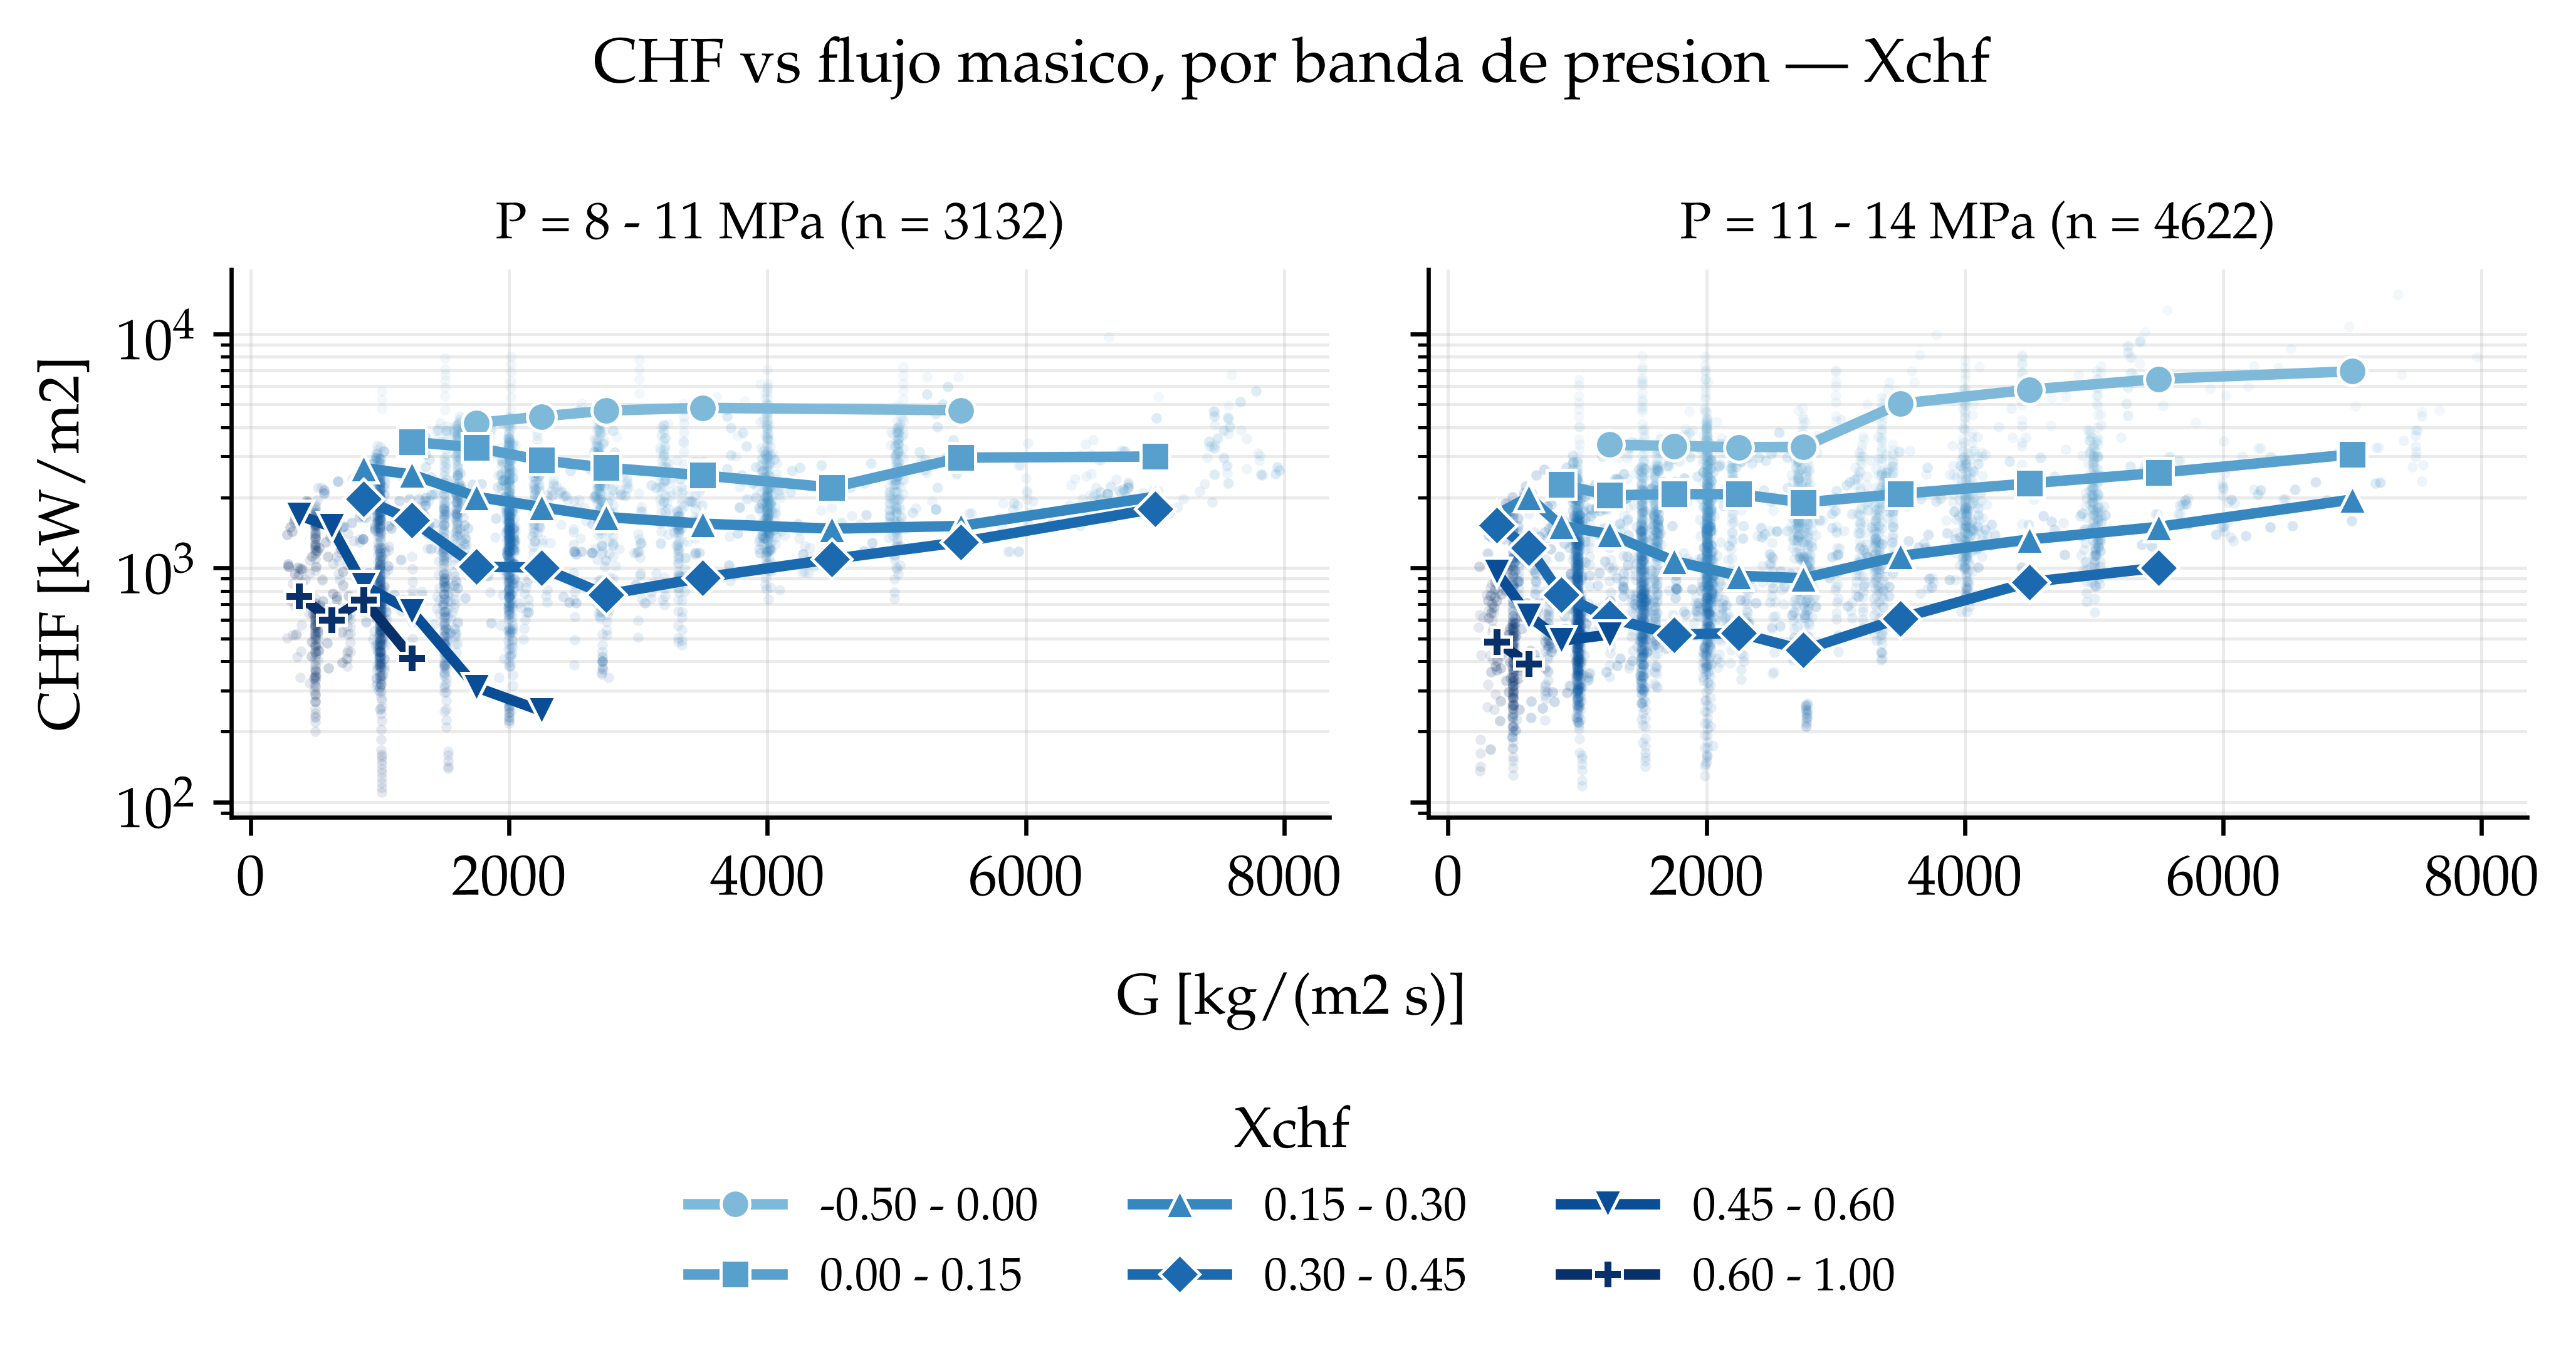
\includegraphics[width=\textwidth]{tendencias_chf_g.png}
\end{frame}

\begin{frame}
    \frametitle{Entrenamiento de la MFPINN}

    Entrenamiento con los puntos obtenidos de COBRA-3CP.
    \vspace{0.5cm}

    \textbf{Problema:} se tiene sólo el mínimo de CHF del ensayo para comparar, y COBRA-3CP obtiene 9060 datos por ensayo. El mínimo hace imposible el entrenamiento por gradiente.
    \begin{itemize}
        \item \textbf{Solución:} entrenamiento con mínimo suave. Se ponderan los puntos con menor predicción de CHF, disminuyendo la cantidad al avanzar las épocas de entrenamiento.
    \end{itemize}
    \vspace{0.5cm}

    \textbf{Evaluación de modelos con penalización:} se entrena con los ensayos de alto caudal y evalúa con los de bajo caudal. Los modelos con correctas relaciones físicas logran generalizar a la región de menor CHF.
\end{frame}

\begin{frame}
    \frametitle{Entrenamiento de la MFPINN}
    Se evaluó el valor de:
    \begin{itemize}
        \item \textbf{La arquitectura de multifidelidad.} Aporta robustez en la predicción en regiones no entrenadas a través de la información de la LFNN.
        \item \textbf{La incorporación de relaciones físicas.} La correcta combinación de ellas permite reducir la incerteza en la predicción. Asegura predicciones consistentes con la física en regiones no entrenadas.
        \item \textbf{La incorporación de variables adicionales.} No se obtuvo beneficio de ellas, incluso se observó que la predicción empeoraba al incorporarlas.
    \end{itemize}

\end{frame}

\begin{frame}
    \frametitle{Entrenamiento de la MFPINN}
    
    \begin{columns}
        \begin{column}{0.5\textwidth}
            \centering
            MFDNN
            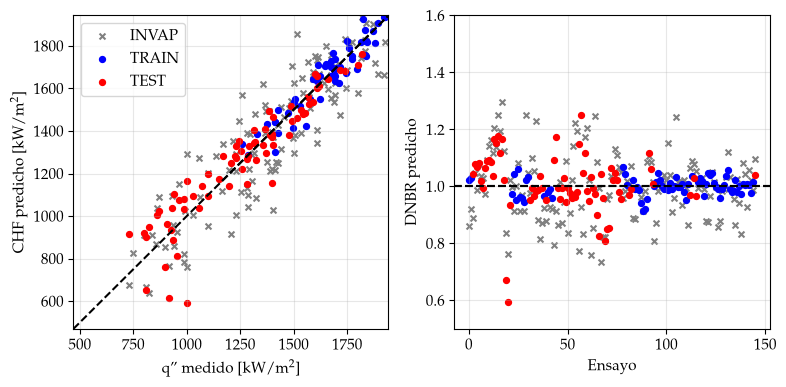
\includegraphics[trim=0 0 280 0,clip,width=0.8\textwidth]{../Figures/chf_mfdnn_pred.png}
            $\mathrm{DNBR}_\mathrm{min} = 1.233$ (*)
        \end{column}
        \begin{column}{0.5\textwidth}
            \centering
            MFPINN
            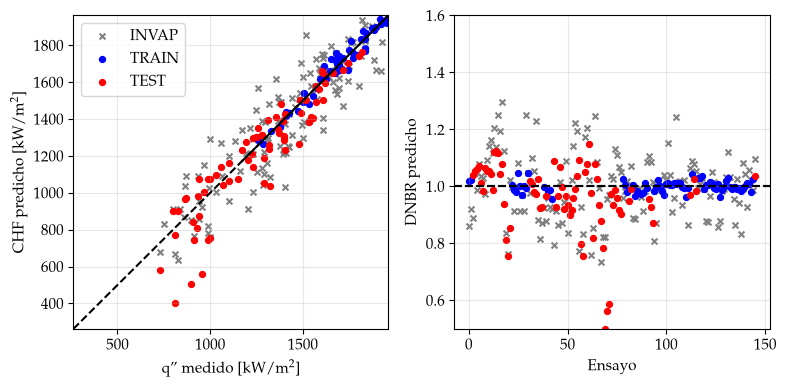
\includegraphics[trim=0 0 280 0,clip,width=0.8\textwidth]{../Figures/chf_mfpinn_E.png}
            $\mathrm{DNBR}_\mathrm{min} = 1.203$ (*)
        \end{column}
    \end{columns}

    \vspace{0.2cm}
    Referencia INVAP: $\mathrm{DNBR}_\mathrm{min} = 1.212$ (sin penalización).

    \vspace{0.2cm}
    \textbf{$\bm{\mathrm{DNBR}_\mathrm{min}}$ en el orden de INVAP pero con modelos penalizados.}

    % \vspace{0.3cm}
    \vspace{0.1cm}
    {\small
        (*) $\mathrm{DNBR}_\mathrm{min}$ obtenido del conjunto de evaluación.
    }
\end{frame}

\begin{frame}
    \frametitle{Predictor de CHF - Modelos finales}

    \begin{columns}
        \begin{column}{0.5\textwidth}
            \centering
            MFDNN
            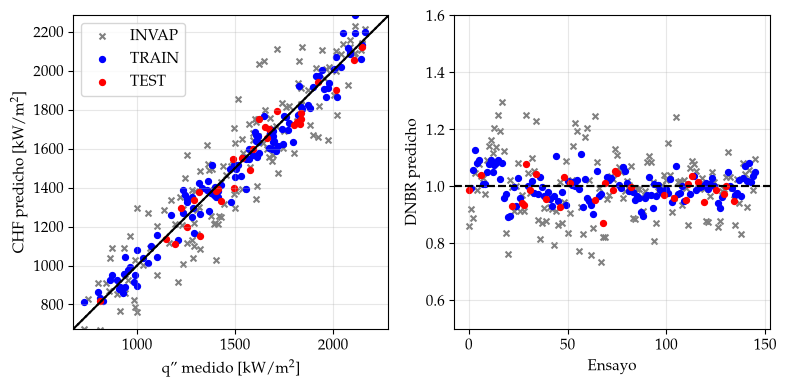
\includegraphics[trim=0 0 280 0,clip,width=0.8\textwidth]{../Figures/chf_mfdnn_pred_final.png}
            $\mathrm{DNBR}_\mathrm{min} = 1.113$ (*)
        \end{column}
        \begin{column}{0.5\textwidth}
            \centering
            MFPINN
            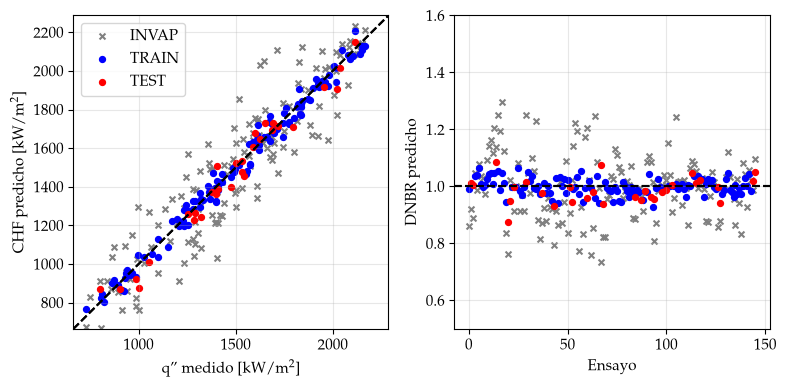
\includegraphics[trim=0 0 280 0,clip,width=0.8\textwidth]{../Figures/chf_mfpinn_pred_final.png}
            $\mathrm{DNBR}_\mathrm{min} = 1.084$ (*)
        \end{column}
    \end{columns}

    \vspace{0.2cm}
    Referencia INVAP: $\mathrm{DNBR}_\mathrm{min} = 1.212$.

    \vspace{0.2cm}
    \textbf{Considerable mejora en $\bm{\mathrm{DNBR}_\mathrm{min}}$ para ambas metodologías.}

    \vspace{0.1cm}
    {\small
        (*) $\mathrm{DNBR}_\mathrm{min}$ obtenido del conjunto de evaluación.
    }
\end{frame}

\begin{frame}
    \frametitle{Predictor de CHF - Evaluación del impacto en PLC}
    \textbf{¿Qué impacto tiene la mejora en $\bm{\mathrm{DNBR}_\mathrm{min}}$ sobre la PLC?}

    % Aumento de PLC por zona hidráulica para la metodología MFPINN, respecto de la metodología de INVAP.

    % Evaluado con los condiciones conservativas del diseño termohidráulico de la CNA-UII.

    \begin{table}[H]
        \centering
        \begin{tabular}{c c c c c c} 
            \toprule
                        & \multicolumn{5}{c}{\textbf{Zona Hidráulica}} \\
                        & 1         & 2         & 3         & 4         & 5         \\ \hline
            Diferencia  & $+2.6\%$  & $+7.6\%$ & $+9.7\%$ & $+3.6\%$ & $+3.0\%$ \\
            \bottomrule
        \end{tabular}
    \end{table}

    Tener en cuenta: 
    \begin{itemize}
        \item Sólo la ZH5 se encuentra limitada por DNBR. Las zonas 1 a 4 están limitadas por la fracción de vacío.
        \item El cambio de metodología de predicción de CHF podría modificar el $\mathrm{SDL}_\mathrm{max}$, impactando en el $\mathrm{DNBR}_\mathrm{LCO}$.
    \end{itemize}

\end{frame}

\section{Conclusiones y trabajo futuro}
\begin{frame}
    \frametitle{Conclusiones y trabajo futuro}
    Objetivos específicos:
    \begin{itemize}[label={\checkmark}]
        \item Herramienta predictiva de PLC.
        \item Análisis de características relevantes de los perfiles de potencia de los elementos combustibles.
        \item Metodología de predicción de CHF para la CNA-UII, basada en IA.
    \end{itemize}

    Objetivos estratégicos:
    \begin{itemize}[label={\checkmark}]
        \item Disminución en entre $2\,000$ y $9\,500$ veces el tiempo de cómputo para estimación de PLC.
        \item Mejora de la predicción de CHF para el bundle de la CNA-UII, obteniendo un $\mathrm{DNBR}_\mathrm{min} = 1.084$ y un posible aumento de PLC de $+3.0\%$.
    \end{itemize}
\end{frame}

\begin{frame}
    \frametitle{Conclusiones y trabajo futuro}
    \textbf{Predictor de PLC:}
    \begin{itemize}[label={\square}]
        \item Análisis de casos anómalos fuera del conjunto de entrenamiento. ¿Es conservativa la extrapolación?
        \item Investigar si se predicen los mismos casos y canales limitantes que con COBRA-3CP.
        \item Analizar mejoras en predicción para zonas periféricas. ¿Es necesario entrenar con aun más sobrepotencia en estas zonas?
        \item Implementar el modelo en un entorno de cálculo real.
    \end{itemize}
\end{frame}

\begin{frame}
    \frametitle{Conclusiones y trabajo futuro}

    \textbf{Predictor de CHF:}
    \begin{itemize}[label={\square}]
        \item Realizar un análisis cuantitativo de los límites de aplicación de las relaciones diferenciales físicas propuestas.
        \item Mejorar el modelo de baja fidelidad, específicamente en el rango de operación de la CNA-UII. ¿Permite mejorar aún más la predicción del modelo MFPINN?
        \item Optimización de hiperparámetros por medio de Optuna.
        \item Implementación del modelo final en COBRA-3CP.
        \item Cálculo del diseño termohidráulico completo para definir el impacto real en PLC.
    \end{itemize}
\end{frame}


\end{document}